% !TEX encoding = UTF-8
% !TEX program = pdflatex
% !TEX spellcheck = it_IT

\documentclass[a4paper, 11pt]{article}

% appendix

\usepackage[toc,page]{appendix}

% sintassi
\usepackage[T1]{fontenc}
\usepackage[utf8]{inputenc}
\usepackage[english]{babel}
\DeclareUnicodeCharacter{00A0}{~}
\usepackage{fullpage}
%\usepackage[cochineal]{newtxmath}
%\usepackage{crimson,verbatim}
\usepackage{textcomp}
\usepackage{color,soul,hyperref,mwe}

% matematica e chimica

\usepackage{siunitx,amsmath,bm,chemfig}
\newcommand{\ud}{\mathop{}\!\mathrm{d}}
\sisetup{detect-all,math-rm = \ensuremath}
%\usepackage{arev}
\usepackage[charter]{mathdesign}


\setatomsep{2em}

\newcommand\setpolymerdelim[2]{\def\delimleft{#1}\def\delimright{#2}} 
\def\makebraces[#1,#2]#3#4#5{% 
\edef\delimhalfdim{\the\dimexpr(#1+#2)/2}% 
\edef\delimvshift{\the\dimexpr(#1-#2)/2}% 
\chemmove{% 
\node[at=(#4),yshift=(\delimvshift)] {$\left\delimleft\vrule height\delimhalfdim depth\delimhalfdim 
width0pt\right.$};% 
\node[at=(#5),yshift=(\delimvshift)] 
{$\left.\vrule height\delimhalfdim depth\delimhalfdim 
width0pt\right\delimright_{\rlap{$\scriptstyle#3$}}$};}} 
\setpolymerdelim()

% tabelle e grafica
\usepackage{booktabs,graphicx,subfig,caption,pdfpages}
\captionsetup{font=small,
	format=hang,
	justification=centering,
	singlelinecheck=true,
	labelfont={sf,bf}	
}
\usepackage{float}
\floatstyle{plaintop}
\restylefloat{table}
\usepackage{multirow}
\usepackage{fancyhdr}
\pagestyle{fancy}
\fancyhead[LE,RO]{\textsl{\rightmark}}
\fancyhead[LO,RE]{\nouppercase{\leftmark}}
\fancyfoot[C]{\thepage}
\usepackage[margin=1in,headsep=.3in]{geometry}
\usepackage[suftesi]{frontespizio}
\usepackage{xparse}
\setlength\parindent{0pt}

\newenvironment{chapterabstract}{%
  \par\nobreak\noindent
  \textbf{\textit{Abstract}\hrulefill}\nobreak
  %\small
  \noindent\ignorespaces
}{%
  \par\nobreak\normalsize
  \vskip-\ht\strutbox\noindent
  \textbf{\hrulefill}%
}
\makeatletter
\NewDocumentCommand\headerspdf{ O {pages=-} m }{% [options for include pdf]{filename.pdf}
  \includepdf[%
    #1,
    pagecommand={\thispagestyle{fancy}},
    scale=1,
    ]{#2}}
\NewDocumentCommand\secpdf{somO{1}m}{% [short title]{section title}[page specification]{filename.pdf} --- possibly starred
  \clearpage
  \thispagestyle{fancy}%
  \includepdf[%
    pages=#4,
    pagecommand={%
      \IfBooleanTF{#1}{%
        \section*{#3}}{%
        \IfNoValueTF{#2}{%
          \section{#3}}{%
          \section[#2]{#3}}}},
    scale=.65,
    ]%
    {#5}}
\makeatother

\begin{document}

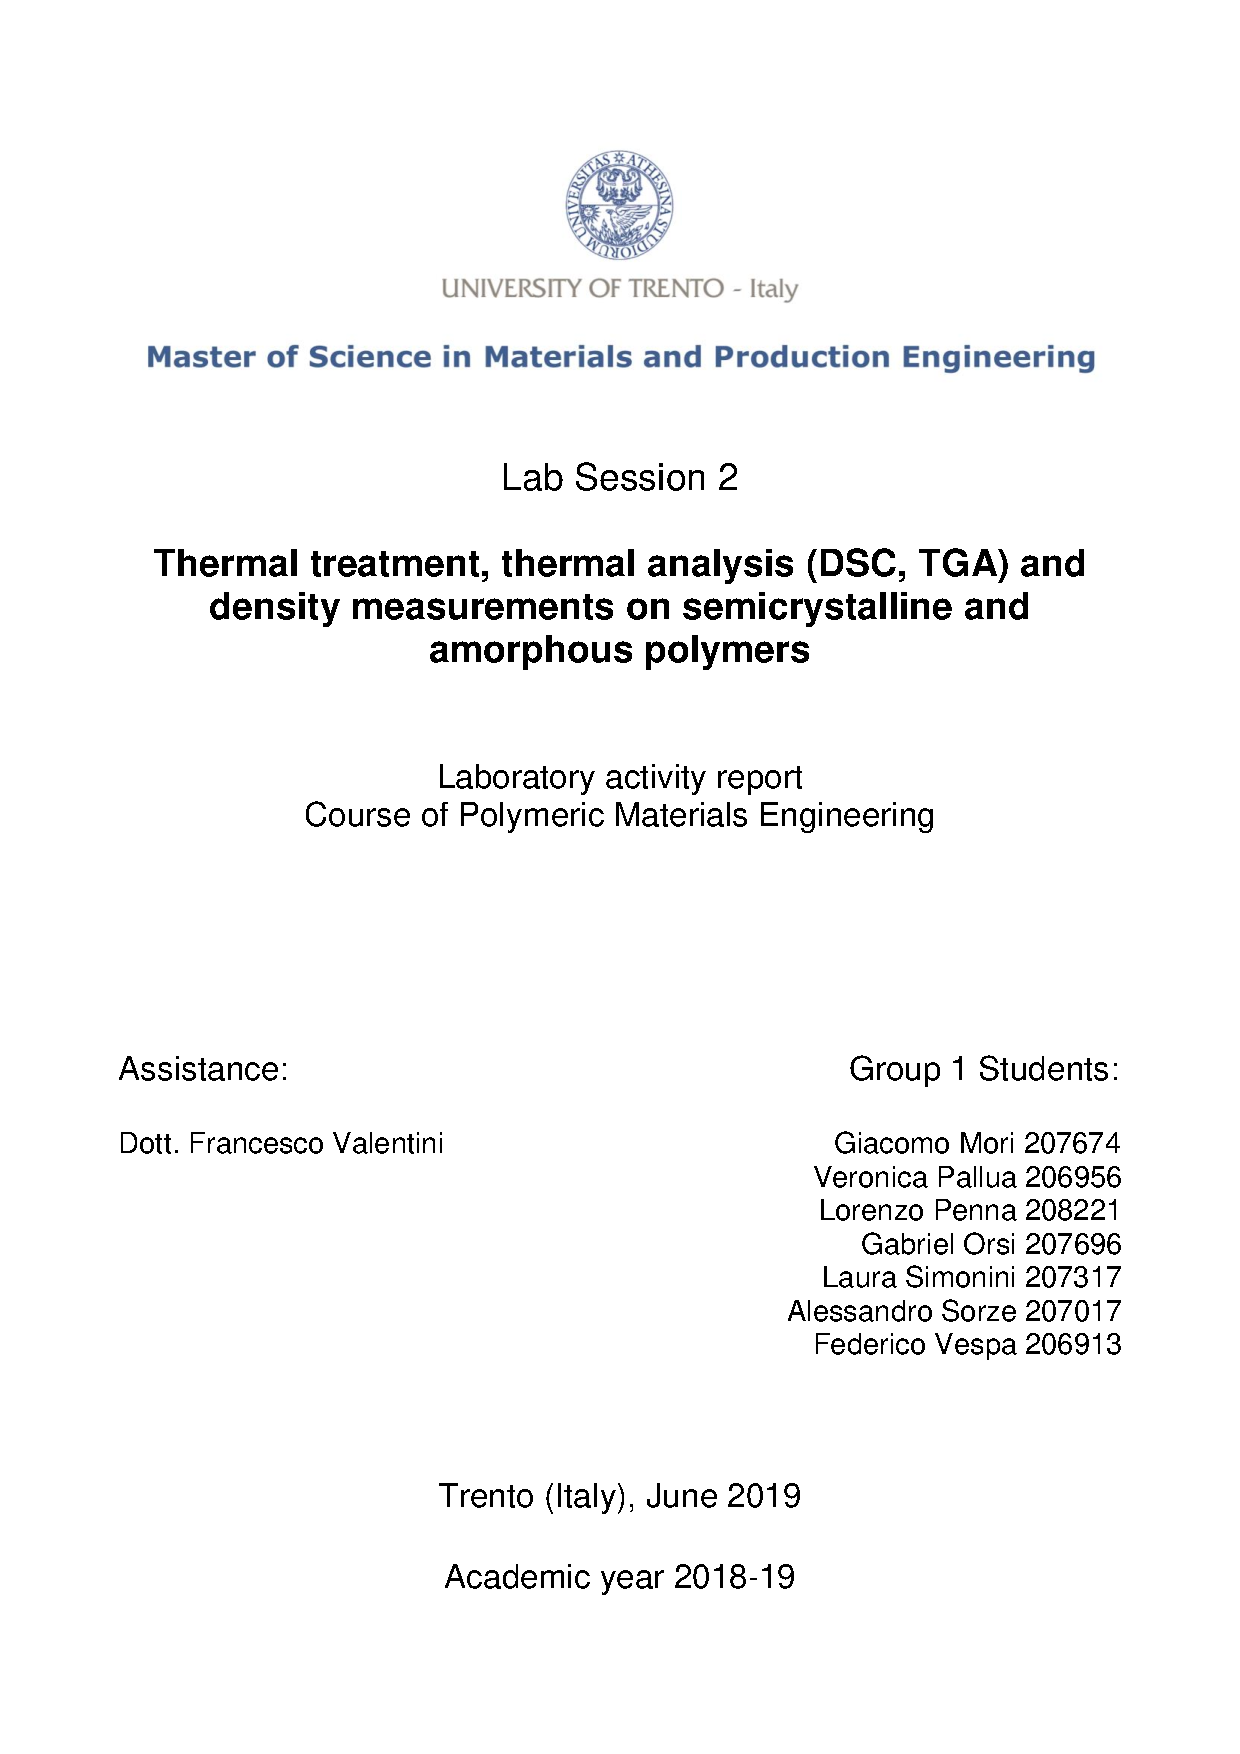
\includepdf[pages=-]{frontespizio2.pdf}

\begin{chapterabstract}

In this work several plastic objects have been studied both thermically and microstructurally: in particular, density measurements, crystallinity measurements, DSC, TGA and solvent effects have been studied. The aim of the work is to find a correlation between thermal properties, crystallinity and stability on heating and solvent attack. 

\end{chapterabstract} 

\section{Introduction}

The laboratory activity concerns the analysis of several polymer materials in PP, PE, PS, PET, PLA, PMMA and tire rubber. PMMA is used referring to bone cement produced in report 1. Endothermic and exothermic transition of samples has been studied and it was also possible to determinate their degree of crystallinity by considerations on specific enthalpy of melting. Density measurements have been carried out, comparing results with theoretical ones and comparing found degree of cristallinity with one of thermal analysis. In order to study directly the thermal behaviour of samples, different heat treatments have been done. Thermal analysis of bone cement and tire rubber has been done in order to study the composition of samples and their residual mass at high temperature. Sample has been treated with solvents of different concentration in order to study their resistance to chemicals.
The various samples used during the activity have been made by different processes. Cups have been produced by thermoforming, in which a plastic sheet is heated to a certain forming temperature, formed to a specific shape in a mold and cut to produce an usable product. 
Coffee sticks and bottle cups have been obtained by injection molding: the polymer is melted in a specif chamber, injected in a mold and then cooled and solidified.
PET bottles have been produced by injection blow molding, a process in which a cylindrical preform is heated and then blown in a mold.

\subsection {Materials}

\subsubsection{Polyethylene}

\begin{figure}[htp]
	\centering
	{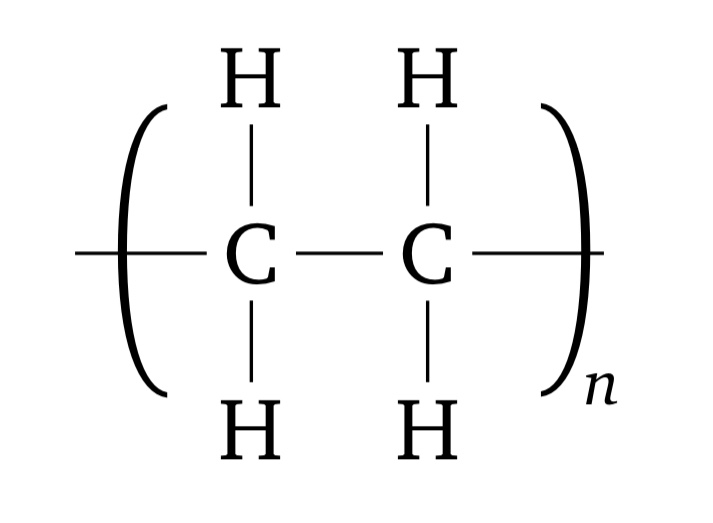
\includegraphics[scale=0.12]{pe_chem}}
	\captionsetup{justification=centering}
	\label{fig:PE}
\end{figure}
PE is a semicrystalline polymer and due to its low glass transition temperature (below room temperature) it shows a certain deformability.
\begin{figure}[htp]
	\centering
	{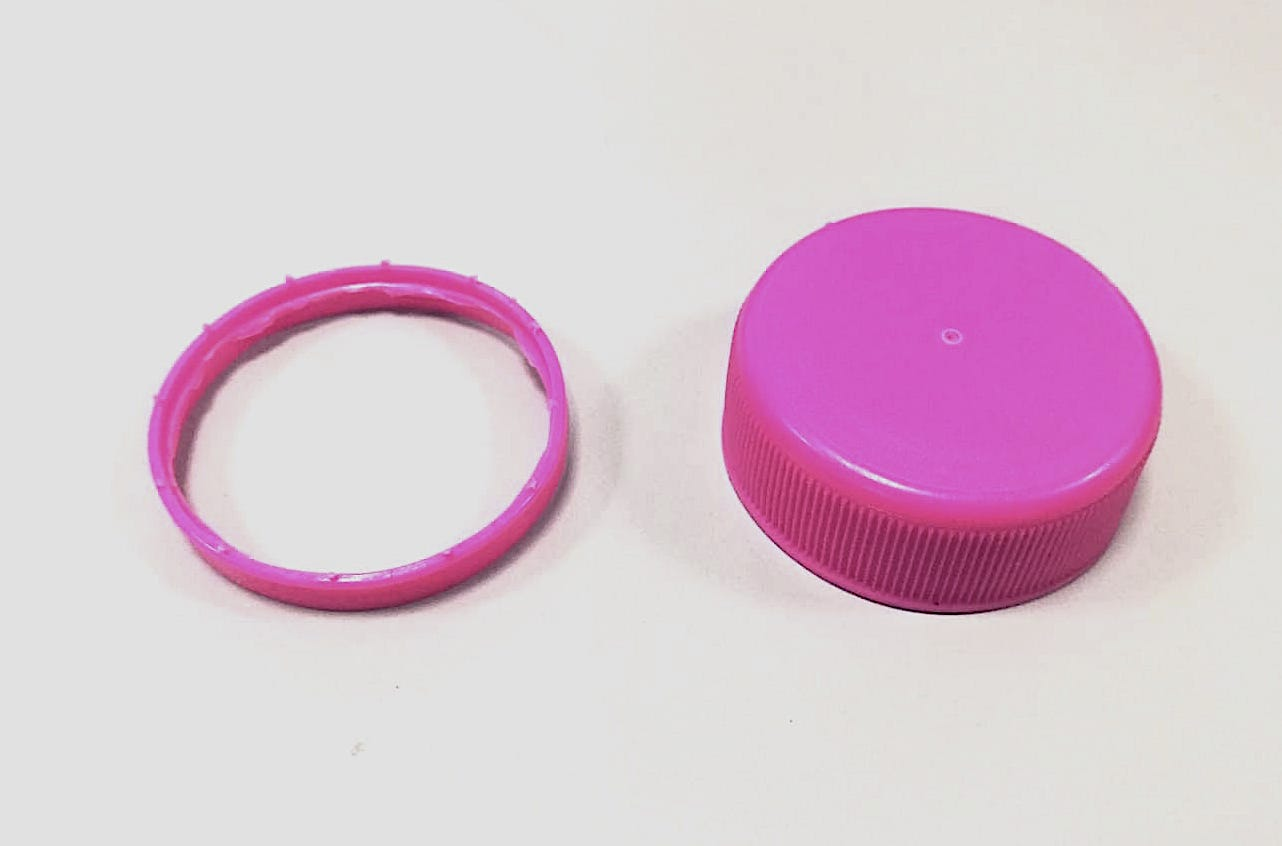
\includegraphics[scale=0.15]{PE}}
	\captionsetup{justification=centering}
	\caption{PE sample.}
	\label{fig:PE}
\end{figure}

\newpage

\subsubsection{Polystyrene}

\begin{figure}[htp]
	\centering
	{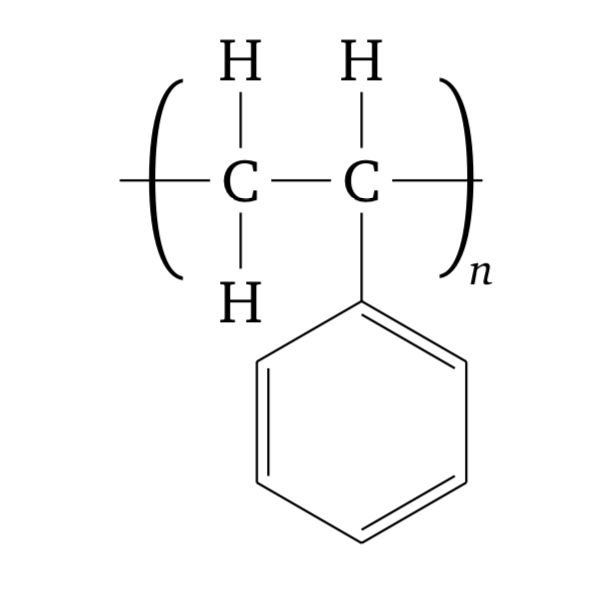
\includegraphics[scale=0.16]{ps_chem}}
	\captionsetup{justification=centering}
	\label{fig:PE}
\end{figure}
PS presents an aromatic ring in his structure that leads to a steric envelope responsable of the low mobility of the chain. Therefore it's an amorphous and rigid polymer in the typically found atactic configuration, known as a-PS.

\begin{figure}[htp]
	\centering
	\subfloat[][]
	{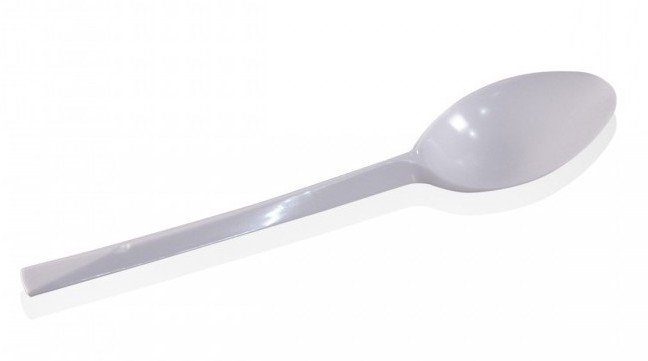
\includegraphics[scale=0.2]{PSspoon}}\qquad
	\subfloat[][]
	{
\includegraphics[scale=0.4]{PS}}
	\captionsetup{justification=centering}
	\caption{PS samples.}
	\label{fig:PS}
\end{figure} 

\subsubsection{Polypropylene}

\begin{figure}[htp]
	\centering
	{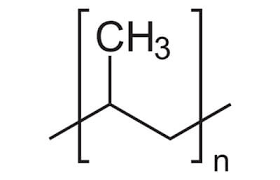
\includegraphics[scale=0.17]{pp_chem}}
	\captionsetup{justification=centering}
	\label{fig:PE}
\end{figure}
PP is a tough and rigid thermoplastic material. Isotactic conformation is obtained by Ziegler-Natta or metallocene polymerization. It shows an high thermal stability due to its semycrystalline structure.

\begin{figure}[h!]
	\centering
	{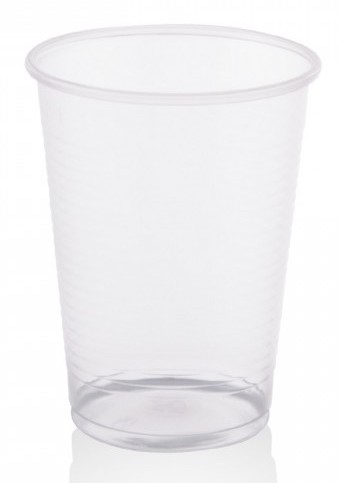
\includegraphics[scale=0.18]{PP}}
	\captionsetup{justification=centering}
	\caption{PP sample.}
	\label{fig:PP}
\end{figure}

\newpage

\subsubsection{Polyethylene terephthalate}

\begin{figure}[htp]
	\centering
	{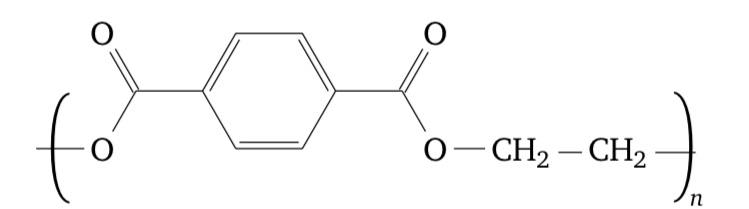
\includegraphics[scale=0.25]{pet_chem}}
	\captionsetup{justification=centering}
	\label{fig:PE}
\end{figure}

PET is a naturally colorless, semi-crystalline material. Some of its most important characteristics include: water resistance, high strength despite low density, shatterproofness and its wide availability as an economic and recyclable plastic.

\begin{figure}[htp]
	\centering
	{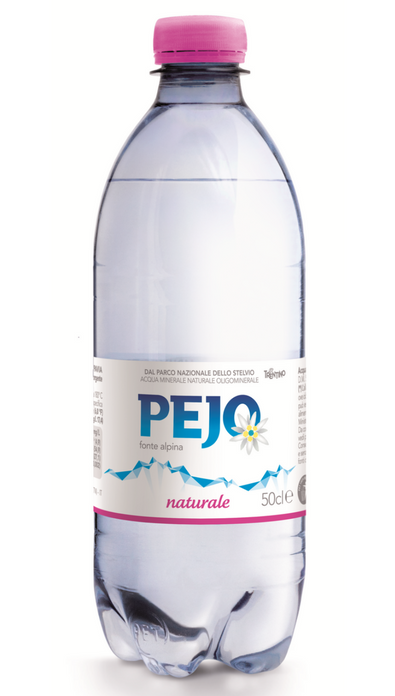
\includegraphics[scale=0.15]{PET}}
	\captionsetup{justification=centering}
	\caption{PET sample.}
	\label{fig:PET}
\end{figure}

\subsubsection{Polyactic acid}

\begin{figure}[htp]
	\centering
	{
\includegraphics[scale=0.3]{pla_chem}}
	\captionsetup{justification=centering}
	\label{fig:PE}
\end{figure}
PLA is an amorphous, biodegradable and bioactive thermoplastic polymer derived from renewable resources like corn starch or sugar cane. It is principally made through condensation and ring-opening polymerization.

\begin{figure}[h!]
	\centering
	{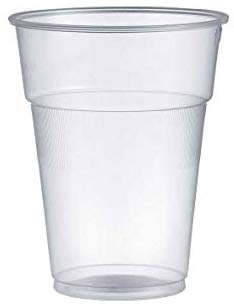
\includegraphics[scale=0.18]{PLA}}
	\captionsetup{justification=centering}
	\caption{PLA sample.}
	\label{fig:PLA}
\end{figure}
 
\subsubsection{Polymethyl methacrylate}

\begin{figure}[h!]
	\centering
	{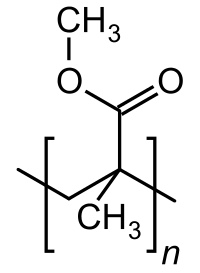
\includegraphics[scale=0.25]{pmma_chem}}
	\captionsetup{justification=centering}
	\label{fig:PE}
\end{figure}
PMMA  is a transparent thermoplastic non-cross linked polymer often used as a lightweight or shatter-resistant alternative to glass.

\newpage 

\section{Materials}

\subsection{Materials}

The polymeric materials that have been used are: plastic yogurt cup (PS), disposable coffee stick (PS), plastic coffee cup (PS), plastic water bottle (PET), plastic bottle cap (PE), plastic cups (PS, PP, PLA), disposable spoon (PS), polymethyl methacrylate (PMMA) bone cement~\cite{gruppo1} and tire piece. In Table \ref{tab:tgtm} main properties of the analyzed polymers are reported. 
\begin{table}[htp]
	\centering
	$
	\begin{array}{lccccc}
	\toprule
	\textbf{Materials} & & \mathbf{Density}\, (\text{g/cm}^3)  & \mathbf{T_{g}} (^\circ\text{C}) \ & \mathbf{T_{m}}(^\circ\text{C}) & \bm{\Delta} \mathbf{H_m} (\text{J/g}) \\
	\midrule
	\text{Polyethylene (PE)} & a & 0.86 & -110 & 138 & 277.1\\
	& c & 1.00 & & & 280.5 \\
	\text{Polystyrene (PS)} & a & 1.04& 100 & - & -  \\
	& c & 1.11 & & 240 & 86.5 \\
	\text{Isotactic polypropylene (i-PP)} & a & 0.85 & -10  & 165  & -\\
	& c & 0.94 & & & 207 \\
	\text{Polyethylene terephthalate (PET)} & a & 1.33 & 70 & 265 & - \\
	& c & 1.51 & & & 140 \\
	\text{Polylactic acid (PLA)} & a & 1.25 & 63 & 178 & -\\
	& c & 1.29 & & & 92.8 \\
	\text{Polymethyl methacrylate (PMMA)} & a & 1.19 & 105  & - & -\\
	\bottomrule
	\end{array}
	$
	\caption{Some properties of used materials where: \\ (a) 100\% amorphous and (c) 100\% crystalline. All values taken from literature~\cite{handbook}.}
	\label{tab:tgtm}
\end{table}\\
Tire samples have been provided by Marangoni (Rovereto (TN), Italy) and are mainly composed by styrene-butadiene rubber (SBR), carbon black, sulfur, accellerators and other additives. All the others objects used in the experimental activity have been provided by University of Trento. \par

The solvents used in this laboratory experience to evaluate the effect on plastics are:
\begin{itemize}
    \item acetone in different concentrations: 25\%, 50\%, 75\% and 100\%;
    \item ethyl alcohol;
    \item mixed solution of ethyl acetate, isopropyl alcohol, aqua, parfum, benzophenonone-1, butyl acetate, glycerin, hydrolyzed keratin, CI 60725 ("\emph{Levasmalto rapido}" by PSS Distribuzione srl, Alessandria (IT));
        \item mixed solution of acetone, aqua, benzophenone, phanthenol, ethyl acetate, parfum, D-limonene, butyl acetate, benzyl alcohol, CI 61565, CI 60725 ("\emph{Levasmalto}" by PSS Distribuzione srl, Alessandria (IT));
    \item mixed solution of methyl acetate, acetone, toluene, xylene, ethyl acetate, heptane, ethyl lactate, methyl formate and methanol ("\textit{Diluente Nitro Antinebbia Top}" by Multichimica Spa, Padova (IT).
\end{itemize}

\newpage

\subsection{Sample preparation}

In Table \ref{tab:code} sample coding is reported. 
\begin{table}[htp]
\centering
$
\begin{tabular}{ll}
\toprule
\textbf{Sample} & \textbf{Description} \\
\midrule
PET & PET without heat treatment, from bottle threaded section \\
PET–T1 & PET with heat treatment T1, from bottle threaded section \\
PET–T2 & PET with heat treatment T2, from bottle threaded section \\
PLA & PLA without heat treatment, from a disposable plastic cup \\
PLA–T1 & PLA with heat treatment T1, from a disposable plastic cup \\
PP & PP taken from a disposable plastic cup \\
PE & PE taken from a plastic bottle cap \\
PS & PS taken from a disposable plastic cup \\
PMMA & bone cement, after soaking for 2 weeks \\
T & tire rubber \\
\bottomrule
\end{tabular}
$
\caption{Sample coding.}
\label{tab:code}
\end{table}\\

Bone cement has been produced in previous laboratory activity from a polymerization reaction between reagents of a medical kit. This kit was constitued of a powder part and a liquid part.

\section{Experimental activity}

\subsection{Heat treatments}

Samples of different types of polymers have been placed into a pressure cooker full of water for 20 minutes (heat treatment T1). In these conditions the samples have been heated at about $120^\circ $C, that corresponds to the boling point of water in the cooker.
Another different treatment that has been carried out is the locally heating of the samples throught a hot air gun (heat treatment T2). In this case the maximun temperature reached is about $150^\circ$C. 
A third treatment has been done by filling the samples with $90^\circ$C hot water (heat treatment T3). 

\subsection{Effect of heat treatments on samples}

Different heat treatments have been done on samples, as reported in Table \ref{tab:heattreatments}. Their effects have been studied, with attention to crystallinity evolution and density. 
\begin{table}[htp]
\centering
$
\begin{tabular}{llll}
\toprule
\textbf{Sample} & \textbf{Description} & \textbf{Duration} & \textbf{Temperature} \\
\midrule
T1 & Pressure cooker soaking & 20 min & 120$^\circ$C \\
T2 & Local heating through hot air gun & 5 min & 150$^\circ$C \\
T3 & Hot water filling & 1 min & 90$^\circ$C \\
\bottomrule
\end{tabular}
$
\caption{Heat treatments.}
\label{tab:heattreatments}
\end{table}\\

\newpage

\subsection{Differential scanning calorimetry (DSC)}

Differential scanning calorimetry (DSC) has been carried out with instrument Mettler DSC30. Samples have been tested in inert nitrogen $100\,\text{ml/min}$ flow, with a heating ramp of $0-300^\circ$C at $20^\circ\text{C/min}$. A first heating is followed by a cooling and eventually by a second heating. This is done in order to reset the thermal hystory of samples and to get informations about the degree of crystallinity (DC). From DSC analysis the specific enthalpy of melting ($\Delta H_m$) and crystallization ($\Delta H_c$) are obtained, together with melting temperature ($T_m$), crystallization temperature ($T_c$), glass transition temperature ($T_g$) and specific heat variation ($\Delta c_p$). 

\subsubsection{Melting enthalpy, degree of crystallinity and density}

Degree of crystallinity ($\alpha_c$) of polymers can be evaluated accordingly to Equation \ref{eq:degreecryst}.
\begin{equation}
\alpha_c = \frac{\Delta H_m - \Delta H_c}{\Delta H_m^{\text{REF}}}
\label{eq:degreecryst}
\end{equation}
Where $\Delta H_c$ is the enthalpy of recrystallization during heating and $\Delta H_m^{\text{REF}}$ is the reference value of specific melting enthalpy of a 100\% crystalline polymer.\\
Density (D) can be extimated knowing the crystallinity of polymers $\alpha_c$, accordingly to empirical Equation \ref{eq:densityemp}.
\begin{equation}
D = D_0+m\cdot \alpha_c
\label{eq:densityemp}
\end{equation}
Where $D_0$ is the density of a completely amorphous polymer while $m$ is the angular coefficient of the interpolating line passing from $D_0$ and the density at 100\% crystallinity. Effect of DEG has been considered in order to calculate the right crystallization degree.

\subsubsection{Effect of DEG in PET}

Melting temperature of PET samples is affected by the presence of diethylene glycole (DEG) accordingly to the Equation \ref{eq:DEG}. See Appendix B for references.
\begin{equation}
T_m = 271-5.25\cdot wt\%_\text{DEG}
\label{eq:DEG}
\end{equation}

\subsection{Density measurements}

The density measurements have been carried out using instrument Gibertini E42. Three samples have been tested: PET, PET–T2 and PET-T3. The normative for this type of test is the ASTM D792~\cite{densità} (Archimedean test), where each specimen has to been weighted in two different conditions, in air and liquid. In particular, for the measurement in the liquid, the sample have been placed inside a container filled with water, using an appropriate plate and mounting. Density of samples has been calculated using Equation \ref{eq:dm}.
\begin{equation}
\rho=\frac{m_{a}}{m_{a}-m_{acq}}\cdot\rho_{w}
\label{eq:dm}
\end{equation}\\
where $m_{a}$ and $m_{acq}$ indicate respectively the mass in air and in water of the specimens and $\rho_{w}$ indicates the water density, measured according to the normative.\\
A comparison with data from the DSC has been done. Having the densities of the samples PET and PET–T2 from Table \ref{tab:dmt} and the crystallinity from Table \ref{tab:handbook}, using the straight line Equation \ref{eq:eqretta} it was possible to calculate the densities of 0\% and 100\% crystalline samples.
\begin{equation}
\rho=\rho_{0}+m\cdot\alpha
\label{eq:eqretta}
\end{equation}
Density measurement of samples of PMMA of the previous lab session were also taking in account. The purpose was to understand how the presence of \chemfig{BaSO_{4}} and water affected the density of the samples, so some specimens of pure PMMA were also considered. The sampling group analyzed was of the polymerization P2 with and without thermal treatment.

\subsection{Thermo-gravimetric analysis (TGA)}

Thermo-gravimetric analysis (TGA) has been carried out with instrument TGA Q5000. Samples have been tested in inert nitrogen $10\,\text{ml/min}$ flow, with a heating ramp of $25-700^\circ$C at $10^\circ\text{C/min}$. Degradation of samples is observed, obtaining the residual mass percent at $700^\circ$C ($m_r$), the onset temperature of degradation ($T_{onset}$) and the temperature of maximum degradation rate ($T_d$). 

\subsection{Solvent effect}

It has been investigated the effect of different solvents on coffee stirrer sticks and on two cups, PS and PP samples. The sticks have been put in test tubes filled with various solvents: acetone with subsequently higher concentrations (25\%, 50\%, 75\%, 100\%); two mixed solutions used in cosmetic field, one with acetone as principal constituent, the other with ethyl acetate and isopropyl alcohol; last solvent employed to test the cups is an aromatic diluent used with paints, this contains various mixture, in particular a percentage of toluene.

\section{Results and discussion}

\subsection{Effect of heat treatments on samples}

Polymers subjected to heat treatments show different behaviours. \\
PP shows poor reactivity to heat during the treatments, due to its crystallinity. PE has not displayed any modification since it is already a semicrystalline polymer at room temperature and its melting point is higher than the temperature reached in this process. PLA has exhibited a process of crystallization since its glass transition has been overcame. Moreover its shape has changed trying to return back to the one before processing. PET has shown the same behaviour of PLA trying to return back to parison shape and crystallizing in its most dense parts (neck and bottom of the bottle). PS samples have been deformed reaching their pre-process plate shape. \\
In the second heat treatment the local heating of samples of PET and PS through the hot air gun has lead to similar results already described for the first treatment. The PE sample, instead, has shown more rubbery behaviour: it could be deformed a lot with high extension of chains due to this local heating. \\ 
In the last heat treatment it has been observed that PLA, as soon as the contact with hot water (about 90°C), has been deformed itself since its $T_{g}$ of 63°C has been overcome. About PP and PS samples nothing has changed since the temperature of water was not so high enough to reach, respectively, their $T_{m}$ and $T_{g}$. In Figure \ref{fig:HT} samples after heat treatments are shown.
\begin{figure}[htp]
\centering
\subfloat[][]
{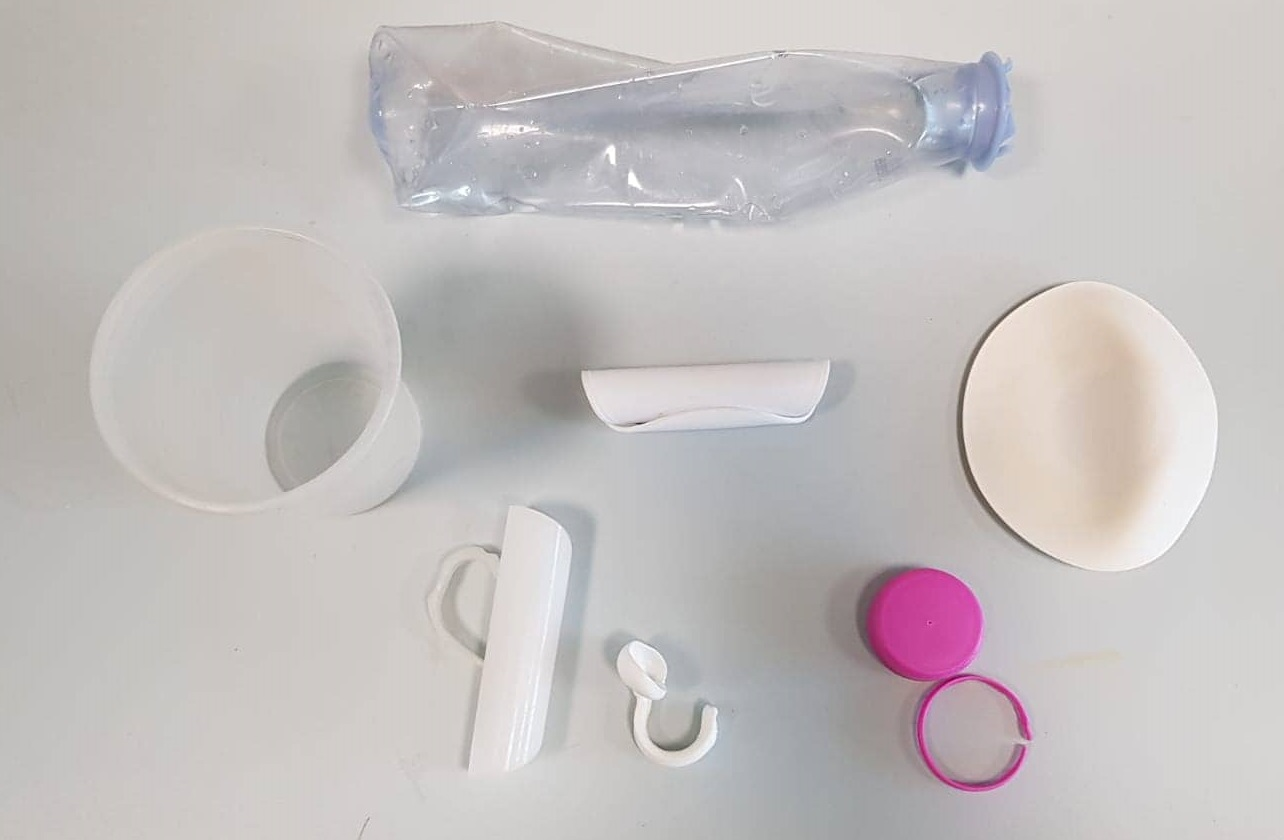
\includegraphics[scale=0.173]{HT1}} \qquad
\subfloat[][]
{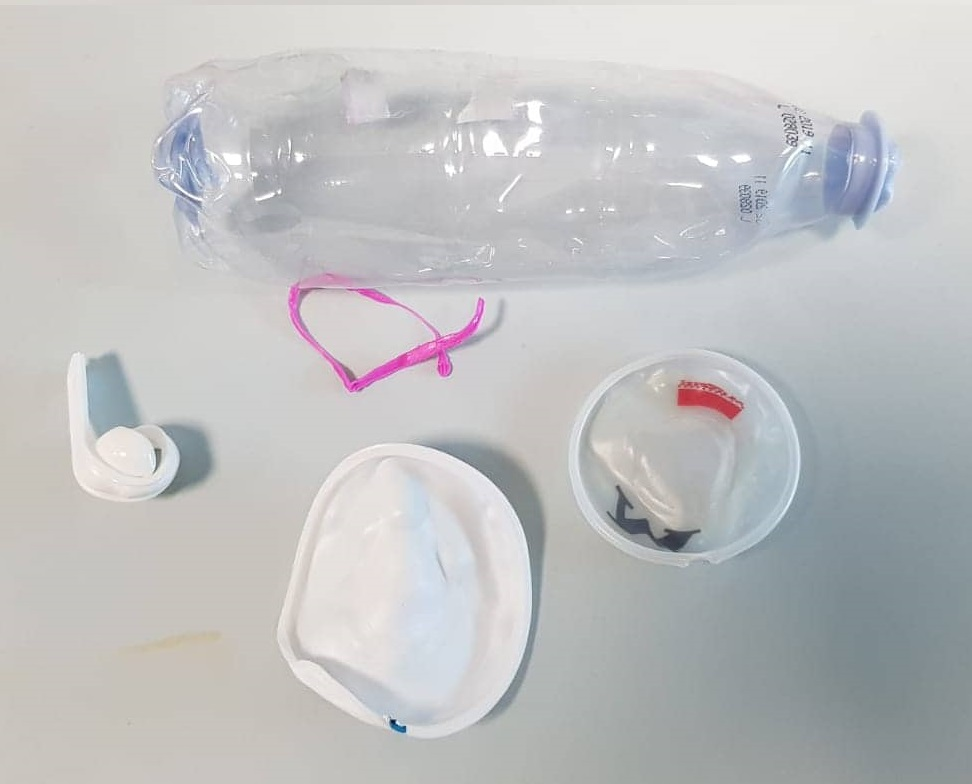
\includegraphics[scale=0.185]{HT2}} \qquad
\subfloat[][]
{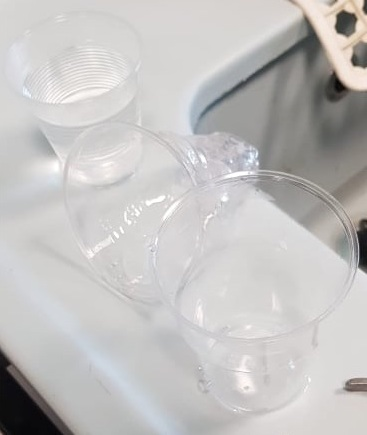
\includegraphics[scale=0.33]{HT3}}
\captionsetup{justification=centering}
\caption{Samples after heat treatments: \\ a) T1, b) T2  c) T3.}
\label{fig:HT}
\end{figure}

\newpage

\subsection{Differential scanning calorimetry (DSC)}

In Figure \ref{fig:dscPET} the DSC thermograms of PET and PET–T2 samples are reported. 
\begin{figure}[htp]
\centering
{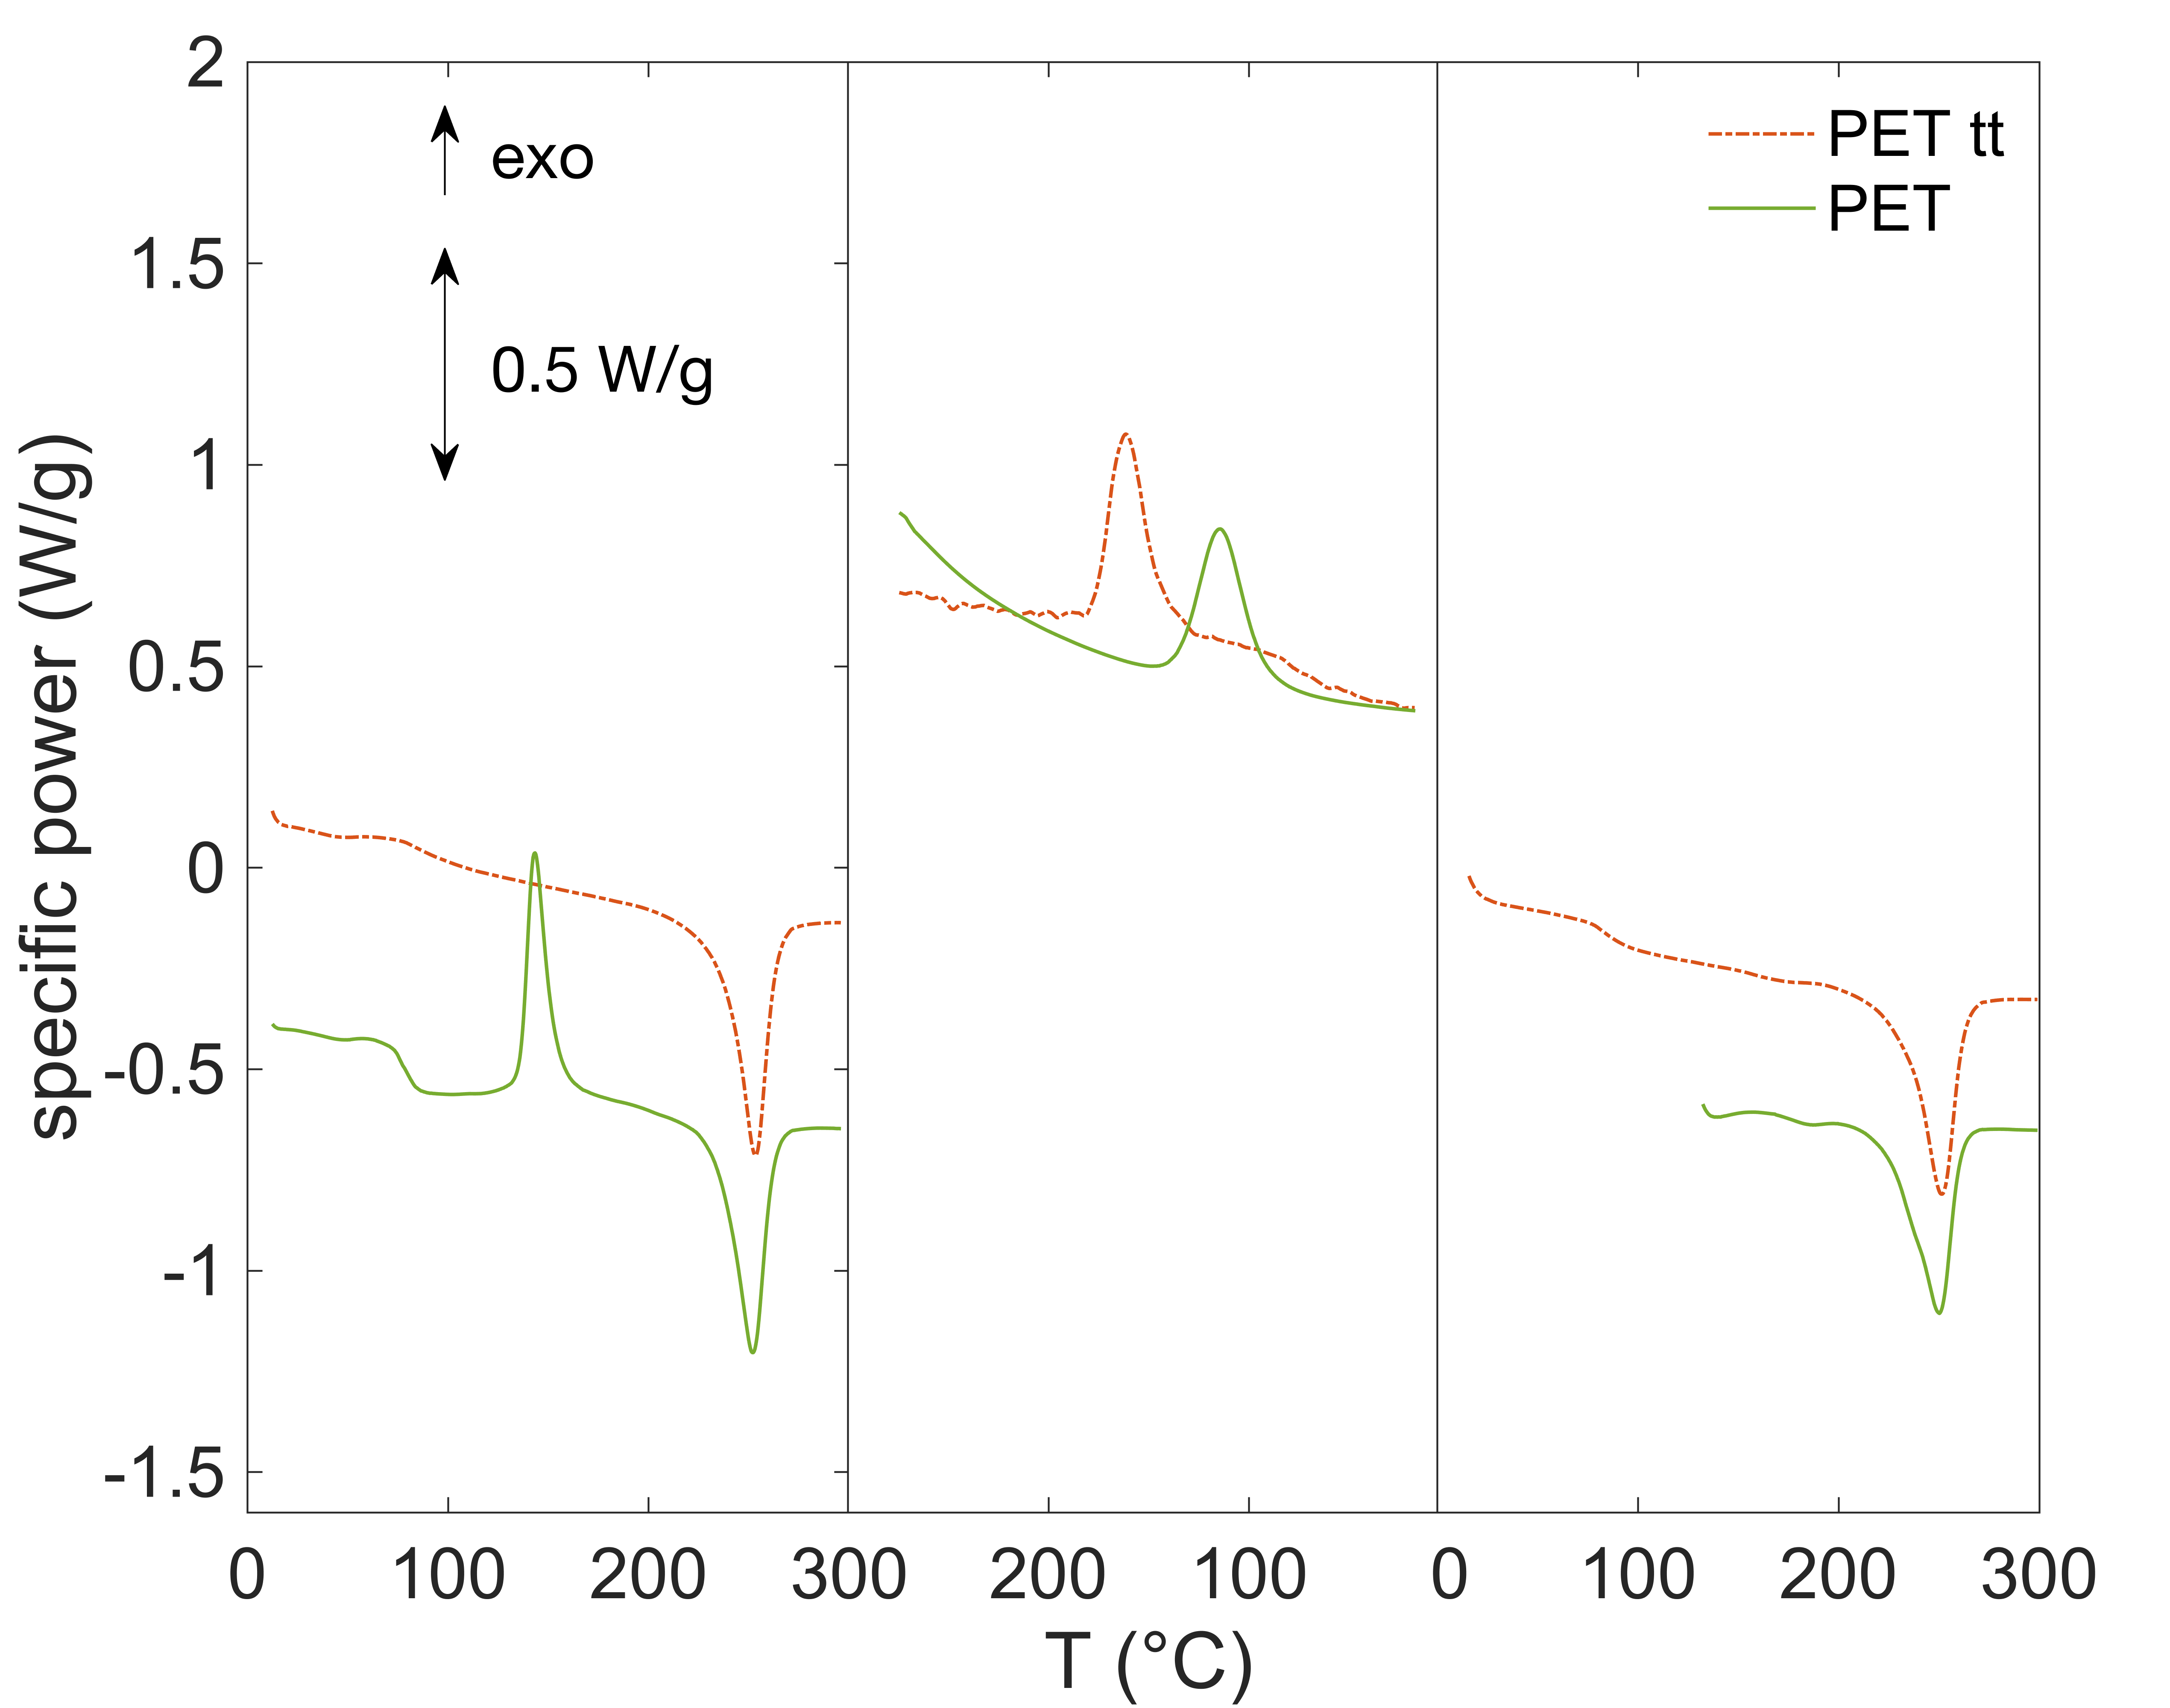
\includegraphics[scale=0.4]{dscPET}} 
\captionsetup{justification=centering}
\caption{DSC thermogram for PET–T2 and PET samples.}
\label{fig:dscPET}
\end{figure}\\
From the analysis the transition temperatures of PET are found. A main difference with reference values for melting temperature (265°C) can be explained by the DEG content. Indeed obtained melting temperature for PET is about $251.8^\circ$C, thus the amount of DEG can be estimated to 3.8\%, accordingly to Equation \ref{eq:DEG}. 
From the chart it can be seen how the heat treated PET doesn't show a crystallization event during the firt heating ramp. This event is related to the completion of crystallization shown by PET on heating, when the mobility of chains is enough for the system to reach a more stable and compact conformation, found in semi-crystalline one. This transformation releases energy since a more stable condition is reached compared to the amorphous one. Both PET–T2 and PET present a melting event but a difference in specific enthalpy of melting is seen: the heat treated sample has an higher value, sign that the grade of crystallinity of it is greater that the non treated PET sample. On cooling, due to an error (run out of nitrogen), the cooling rate is lower than expected and the crystallization of PET sample is delayed with respect to PET–T2. Resulting values of specific crystallization enthalpy are found to be equal on cooling, as the thermal hystory of polymers has been canceled. For same procedural error as before, the second heating ramp starts later, at around 100°C, but both samples are seen to have comparable melting specific enthalpies, while no crystallization events are observed, as the polymer completely crystallized on cooling ramp. 
\newpage

In Figure \ref{fig:dscPP} the DSC thermograms of PE, PP and PS samples are reported. 
\begin{figure}[htp]
\centering
{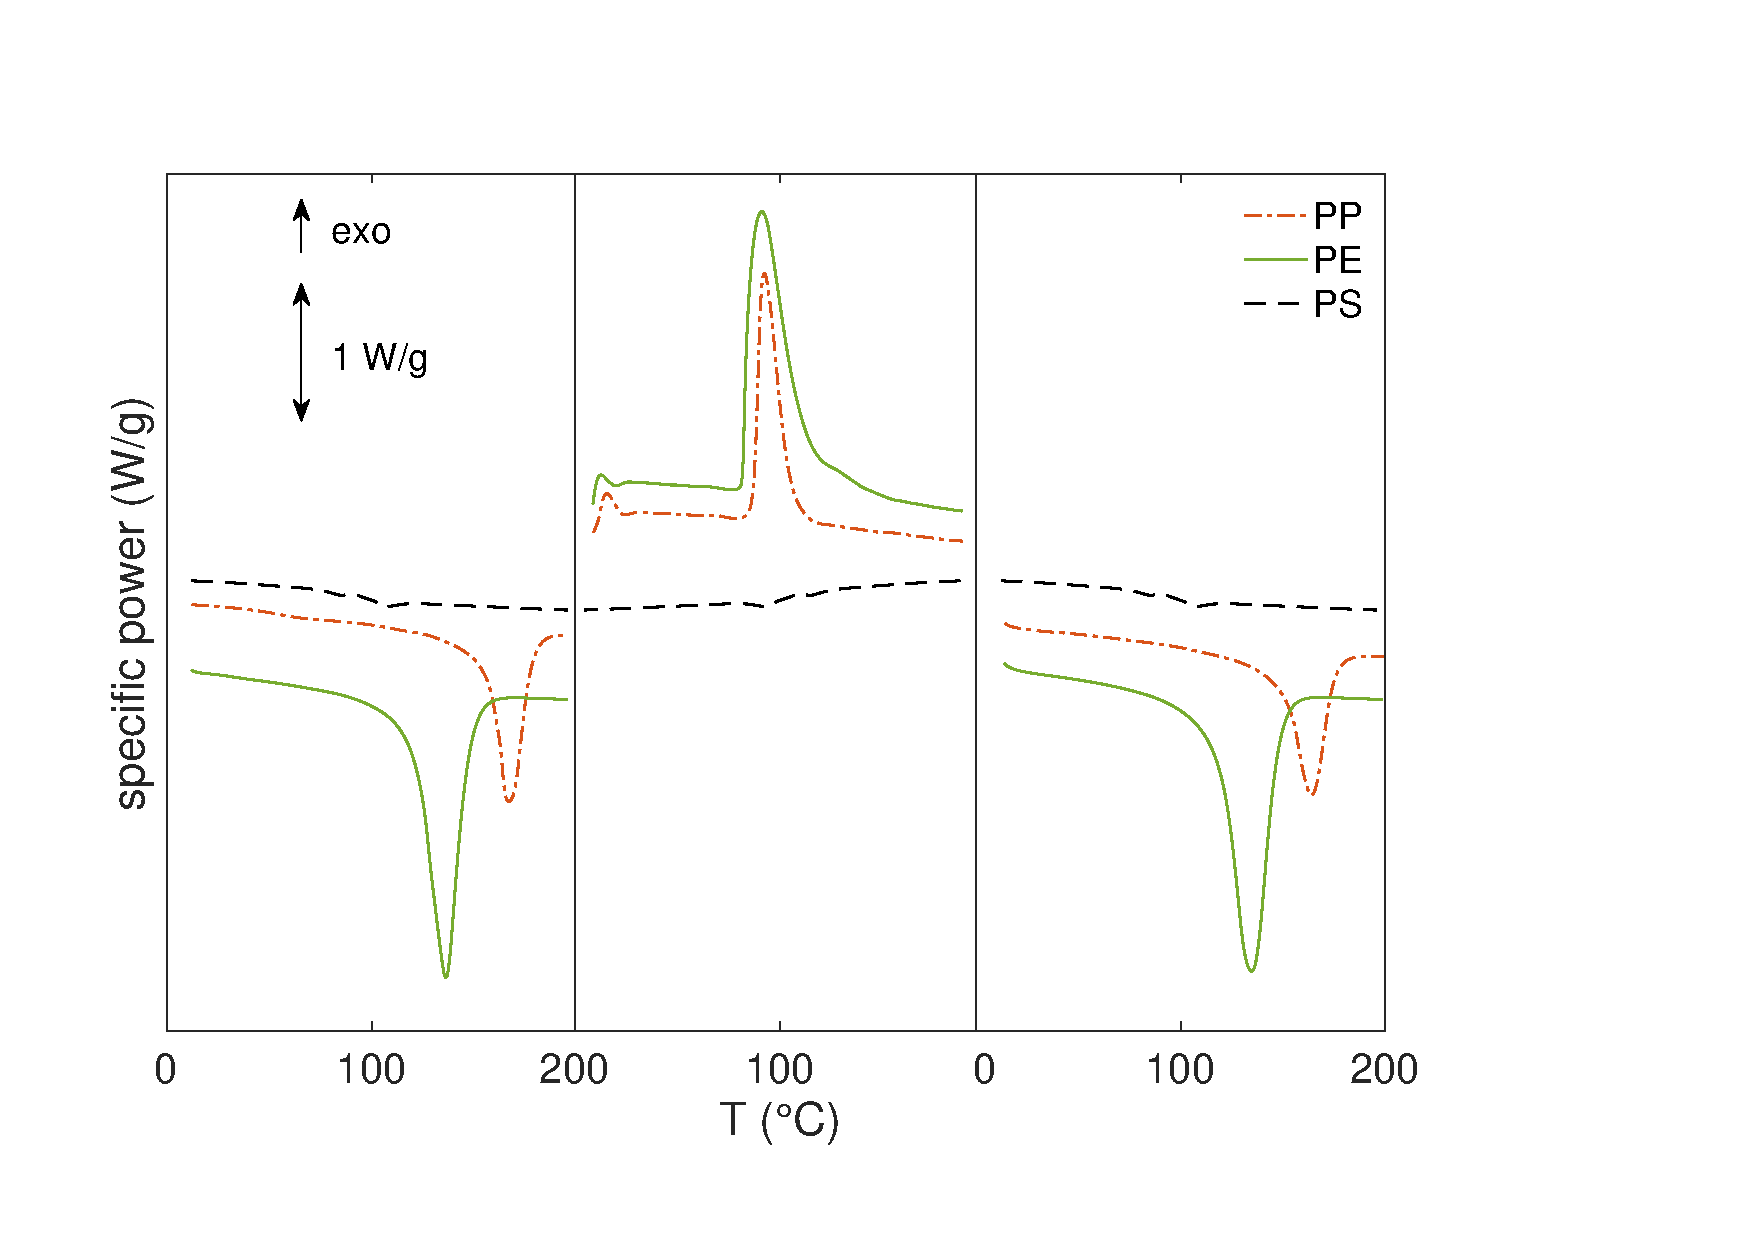
\includegraphics[scale=0.4]{dscPP}} 
\captionsetup{justification=centering}
\caption{DSC thermogram for PE, PP and PS samples.}
\label{fig:dscPP}
\end{figure}\\
In the chart it can be seen how PS shows only glass transition signals, since it's completely amorphous. Glass transition is instead observed either on heating and on cooling. PP and PE present very similar behavior with temperature: both present melting and crystallization while their glass transition temperatures are out of scale (below 0°C) and thus not observed in the analysis. PE is found to release and absorb a lot of energy during respectively crystallization and melting.  \\
In Figure \ref{fig:dscPLA} the DSC thermograms of PLA–T1 and PLA samples is reported. 
\begin{figure}[htp]
\centering
{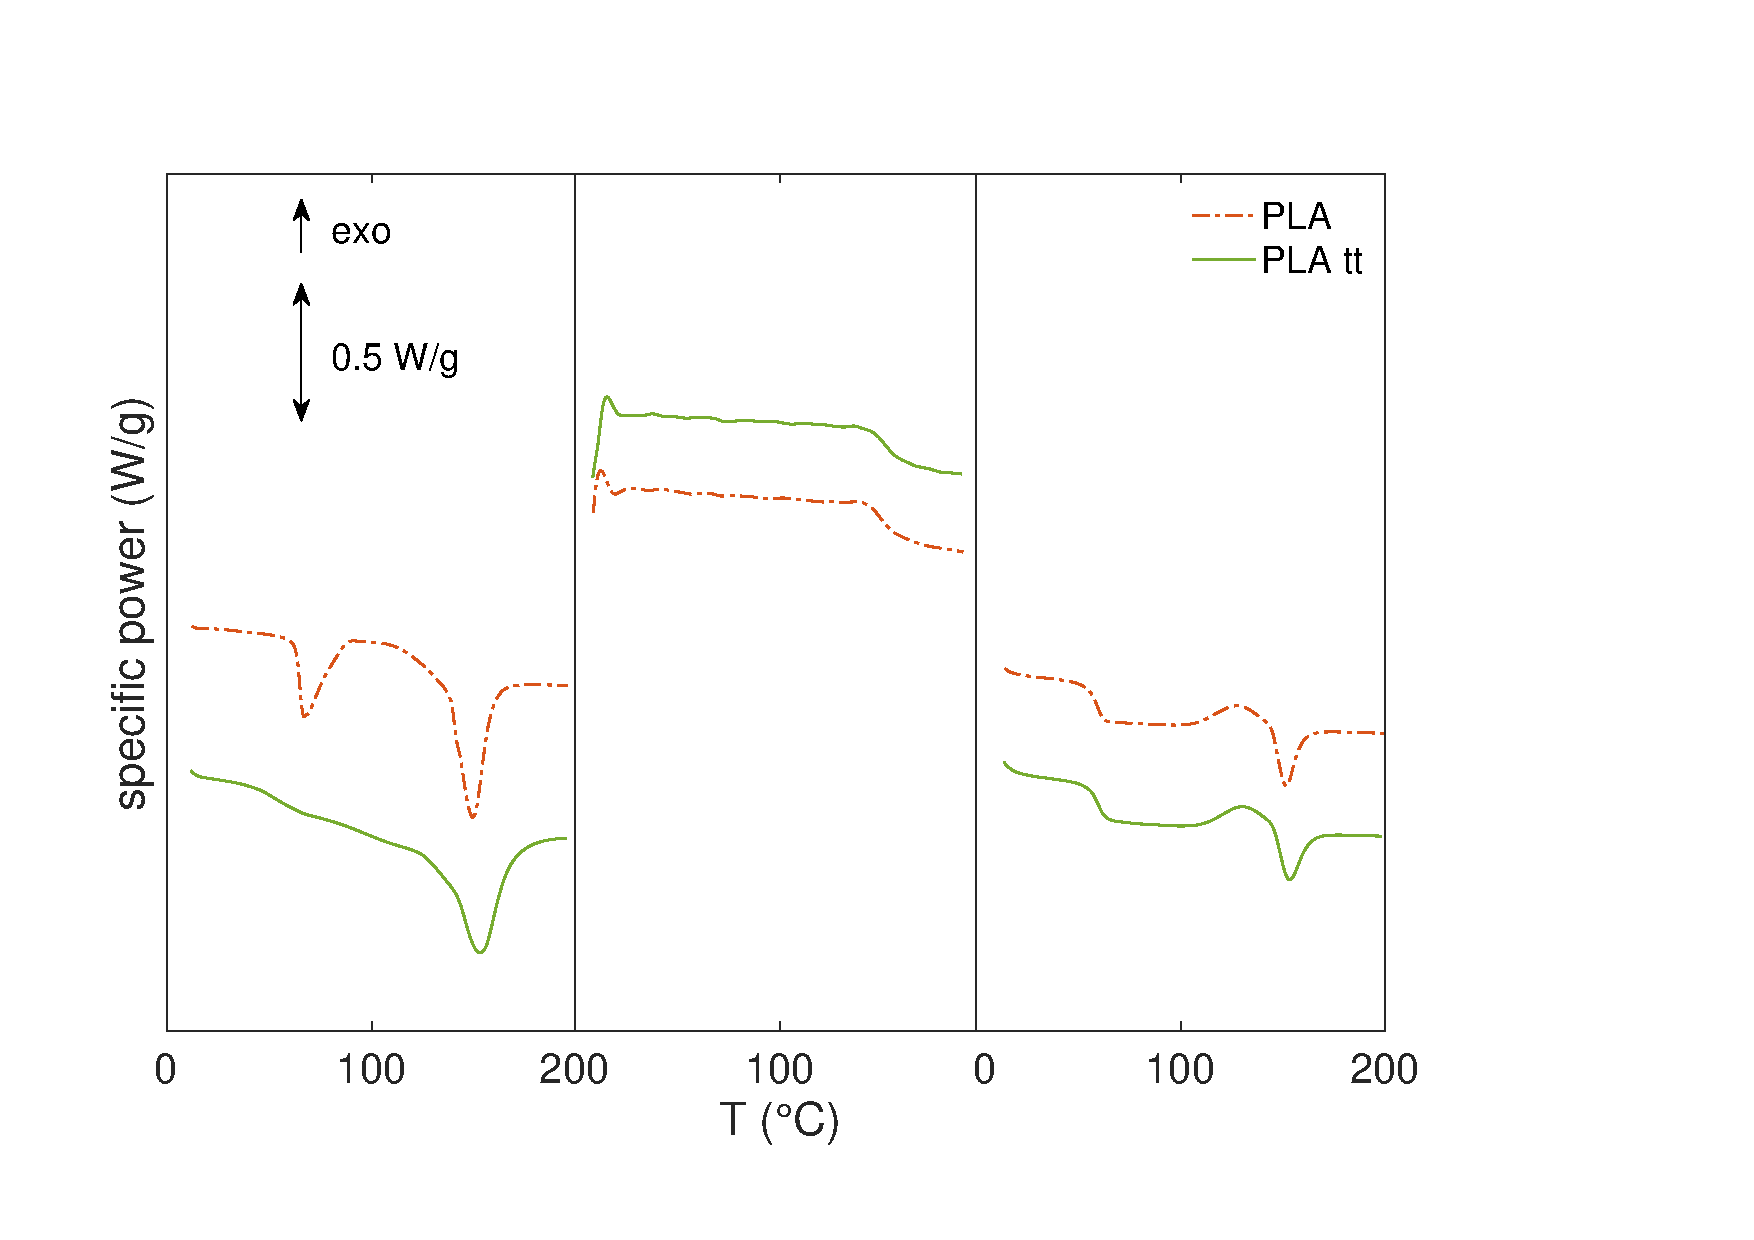
\includegraphics[scale=0.4]{dscPLA}} 
\captionsetup{justification=centering}
\caption{DSC thermogram for PLA–T1 and PLA samples.}
\label{fig:dscPLA}
\end{figure}\\
From the chart it can be seen how the heat treatment in sample PLA–T1 is related to the disappearance of the crystallization event instead present in sample PLA at about $90^\circ$C. Glass transition is observed in both samples together with melting. A significant difference in the specific enthalpy of melting between these samples is observed: PLA–T1 shows a higher value with respect to PLA, evidence that the crystallization occurred during the heat treatment led to an higher level of degree of crystallization. No crystallization events can be seen on cooling, due to the high amount of time required for this polymer in order to crystallize. During second heating ramp, the behavior of PLA and PLA–T1 is the same as the thermal hystory of both samples has been reset.

\newpage

In Table \ref{tab:dsc1} results of DSC analysis of the first heating on all samples are displayed. 
\begin{table}[htp]
\centering
$
\begin{array}{lccccc}
\toprule
\textbf{Sample} & \bm{T_{g}} (\SI{}{\celsius}) & \bm{T_{c}} (\SI{}{\celsius}) & \bm{T_m} (\SI{}{\celsius}) & \bm{\Delta H_{c}} (\si{J/g}) & \bm{\Delta H_m} (\si{J/g}) \\
\midrule
\text{PET} & 76.1 & 143.4 & 251.8 & 23.9 & 35.4 \\
\text{PET–T2} & 82.4 & - & 253.0 & - & 41.2 \\
\text{PLA} & 64.8 & 90.4 & 149.2 & 26.0 & 21.3  \\
\text{PLA–T1} & 50.8 & - & 152.8 & - & 33.9 \\
\text{PE} & - & - & 136.2 & - & 169.6  \\
\text{PP} & - & - & 166.9 & - & 83.0  \\
\text{PS} & 104.5 & - & - & - & -  \\
\bottomrule
\end{array}
$
\caption{DSC results for all samples during the first heating.}
\label{tab:dsc1}
\end{table}\\
In Table \ref{tab:dsc2} results of DSC analysis of the cooling on all samples are displayed. 
\begin{table}[htp]
\centering
$
\begin{array}{lccc}
\toprule
\textbf{Sample} & \bm{T_{g}} (\SI{}{\celsius}) & \bm{T_{c}} (\SI{}{\celsius}) & \bm{\Delta H_{c}} (\si{J/g}) \\
\midrule
\text{PET} & \text{n.d.} & 114.0 & 30.7  \\
\text{PET–T2} & \text{n.d.} & 161.3 & 30.7 \\
\text{PLA} & 52.4 & - & -  \\
\text{PLA–T1} & 49.7 & - & -  \\
\text{PE} & - & 108.7 & 182.4   \\
\text{PP} & - & 107.5 & 83.0   \\
\text{PS} & 86.8 & - & -  \\
\bottomrule
\end{array}
$
\caption{DSC results for all samples during cooling. \\n.d. = not detectable.}
\label{tab:dsc2}
\end{table}\\
In Table \ref{tab:dsc3} results of DSC analysis of the second heating on all samples are displayed. 
\begin{table}[htp]
\centering
$
\begin{array}{lccccc}
\toprule
\textbf{Sample} & \bm{T_{g}} (\SI{}{\celsius}) & \bm{T_{c}} (\SI{}{\celsius}) & \bm{T_m} (\SI{}{\celsius}) & \bm{\Delta H_{c}} (\si{J/g}) & \bm{\Delta H_m} (\si{J/g}) \\
\midrule
\text{PET} & - & - & 250.3 & - & 31.9 \\
\text{PET–T2} & 81.4 & - & 251.1 & - & 34.8 \\
\text{PLA} & 59.3 & 128.7 & 151.6 & 7.5 & 6.1 \\
\text{PLA–T1} & 59.7 & 130.8 & 153.3 & 6.8 & 6.6 \\
\text{PE} & - & - & 134.6 & - & 182.3 \\
\text{PP} & - & - & 164.1 & - & 84.5 \\
\text{PS} & 92.3 & - & - & - & - \\
\bottomrule
\end{array}
$
\caption{DSC results for all samples during the second heating.}
\label{tab:dsc3}
\end{table}

\newpage

\subsubsection{Melting enthalpy, degree of crystallinity and density}

Reported values of melting enthalpy for PET, PLA, PE and PP are compared to reference values found in literature~\cite{handbook}, contained in Table \ref{tab:handbook}, considering completely crystallized polymers.
\begin{table}[htp]
\centering
$
\begin{array}{lcccc}
\toprule
\textbf{Sample} & \bm{\Delta H_m^\text{REF}} (\si{J/g})  & \bm{\Delta H_m} (\si{J/g})  & \bm{\alpha_c} \,(\%) & \bm{D}\, (\si{g/cm^3}) \\
\midrule
\text{PET} & 145 & 11.5 & 8 & 1.35 \\
\text{PET–T2} & 145 & 41.2 & 28 & 1.39 \\
\text{PLA} & 93.6 & 4.7 & 5 & 1.25\\
\text{PLA–T1} & 93.6 & 33.9 & 36 & 1.29\\
\text{PE} & 293 & 169.6 & 58 & 0.94\\
\text{PP} & 207 & 83.0 & 40 & 0.89 \\
\bottomrule
\end{array}
$
\caption{Crystallization degree and density obtained from DSC analyis.}
\label{tab:handbook}
\end{table}\\
Values of density can be extimated knowing the degree of crystallinity of polymers, relating to reference values found in literature~\cite{handbook}, using linear interpolation. 

\subsection{Density measurements}

The water temperature has been measured  obtaining a value of 22.6$^\circ$C, so the water density used is 997.6351$\, \text{kg/m}^{3}$. For each sample, three specimens have been tested. Results for each sample are reported in Table \ref{tab:dmt}. 
\begin{table}[htp]
\centering
$
\begin{array}{lcc}
\toprule
\textbf{Sample} & \boldsymbol{\rho}\,\,({kg/m^{3}})\\
\midrule
\text{PET} & 1313\pm 6\\
\text{PET–T2} & 1336\pm 3 \\
\text{PET-T3} & 1327\pm 3 \\
\bottomrule
\end{array}
$
\caption{Density measurements of PET bottles with different thermal treatment.}
\label{tab:dmt}
\end{table}\\
This values can be compared with the ones obtained by literature~\cite{handbook}, reported in Table \ref{tab:dh}:
\begin{table}[htp]
\centering
$
\begin{array}{lc}
\toprule
\textbf{Cristallinity} & \boldsymbol{\rho}\,\,({kg/m^{3}})\\
\midrule
\text{Amorphus, non-oriented} & 1335\\
\text{Calculated, crystal} & 1515 \\
\bottomrule
\end{array}
$
\caption{Density of PET from literature~\cite{handbook}.}
\label{tab:dh}
\end{table}

It can be observed that the amorphus PET density is different from the one calculated by Archimedean test. This can be explained by the presence of a certain amount of diethylene glycol (DEG), confirmed by DSC analysis, which increases the volume of samples by reducing the density. Starting from a different polymer with respect to the literature one, new values of density for totally crystalline and totally amorphus PET have been calculated. From Equation \ref{eq:eqretta} results are shown in Table \ref{tab:cdm}.
\begin{table}[htp]
\centering
$
\begin{array}{lcc}
\toprule
\textbf{Sample} & \boldsymbol{\alpha}\,(\%) & \boldsymbol{\rho}\,\,({kg/m^{3}})\\
\midrule
\text{Amorphus, non-oriented} & 0 & 1304 \pm 10\\
\text{PET} & 8 & 1313 \pm 6\\
\text{PET–T2} & 28 & 1336 \pm 3\\
\text{Calculated, crystal} & 100 & 1419 \pm 36\\
\bottomrule
\end{array}
$
\caption{Density and crystallinity of PET sample, considering the effect of DEG.}
\label{tab:cdm}
\end{table}\\
\newpage
The density values of the PMMA samples are reported in Table \ref{tab:pmma}.
\begin{table}[htp]
\centering
$
\begin{array}{lc}
\toprule
\textbf{Sample} & \mathbf{\rho}\,\,({kg/m^{3}})\\
\midrule
\text{Pure} & 1183 \pm 1\\
\text{P2} & 1234 \pm 12\\
\text{P2-HT} & 1242 \pm 15\\
\bottomrule
\end{array}
$
\caption{Density of PMMA samples.}
\label{tab:pmma}
\end{table}\\
As the table shows, the density is increased by the presence of \chemfig{BaSO_{4}}.

\subsection{Thermo-gravimetric analysis (TGA)}

In Figure \ref{fig:tga}a-b the TGA thermograms of PMMA and T samples are reported. 
\begin{figure}[htp]
\centering
\subfloat[][]
{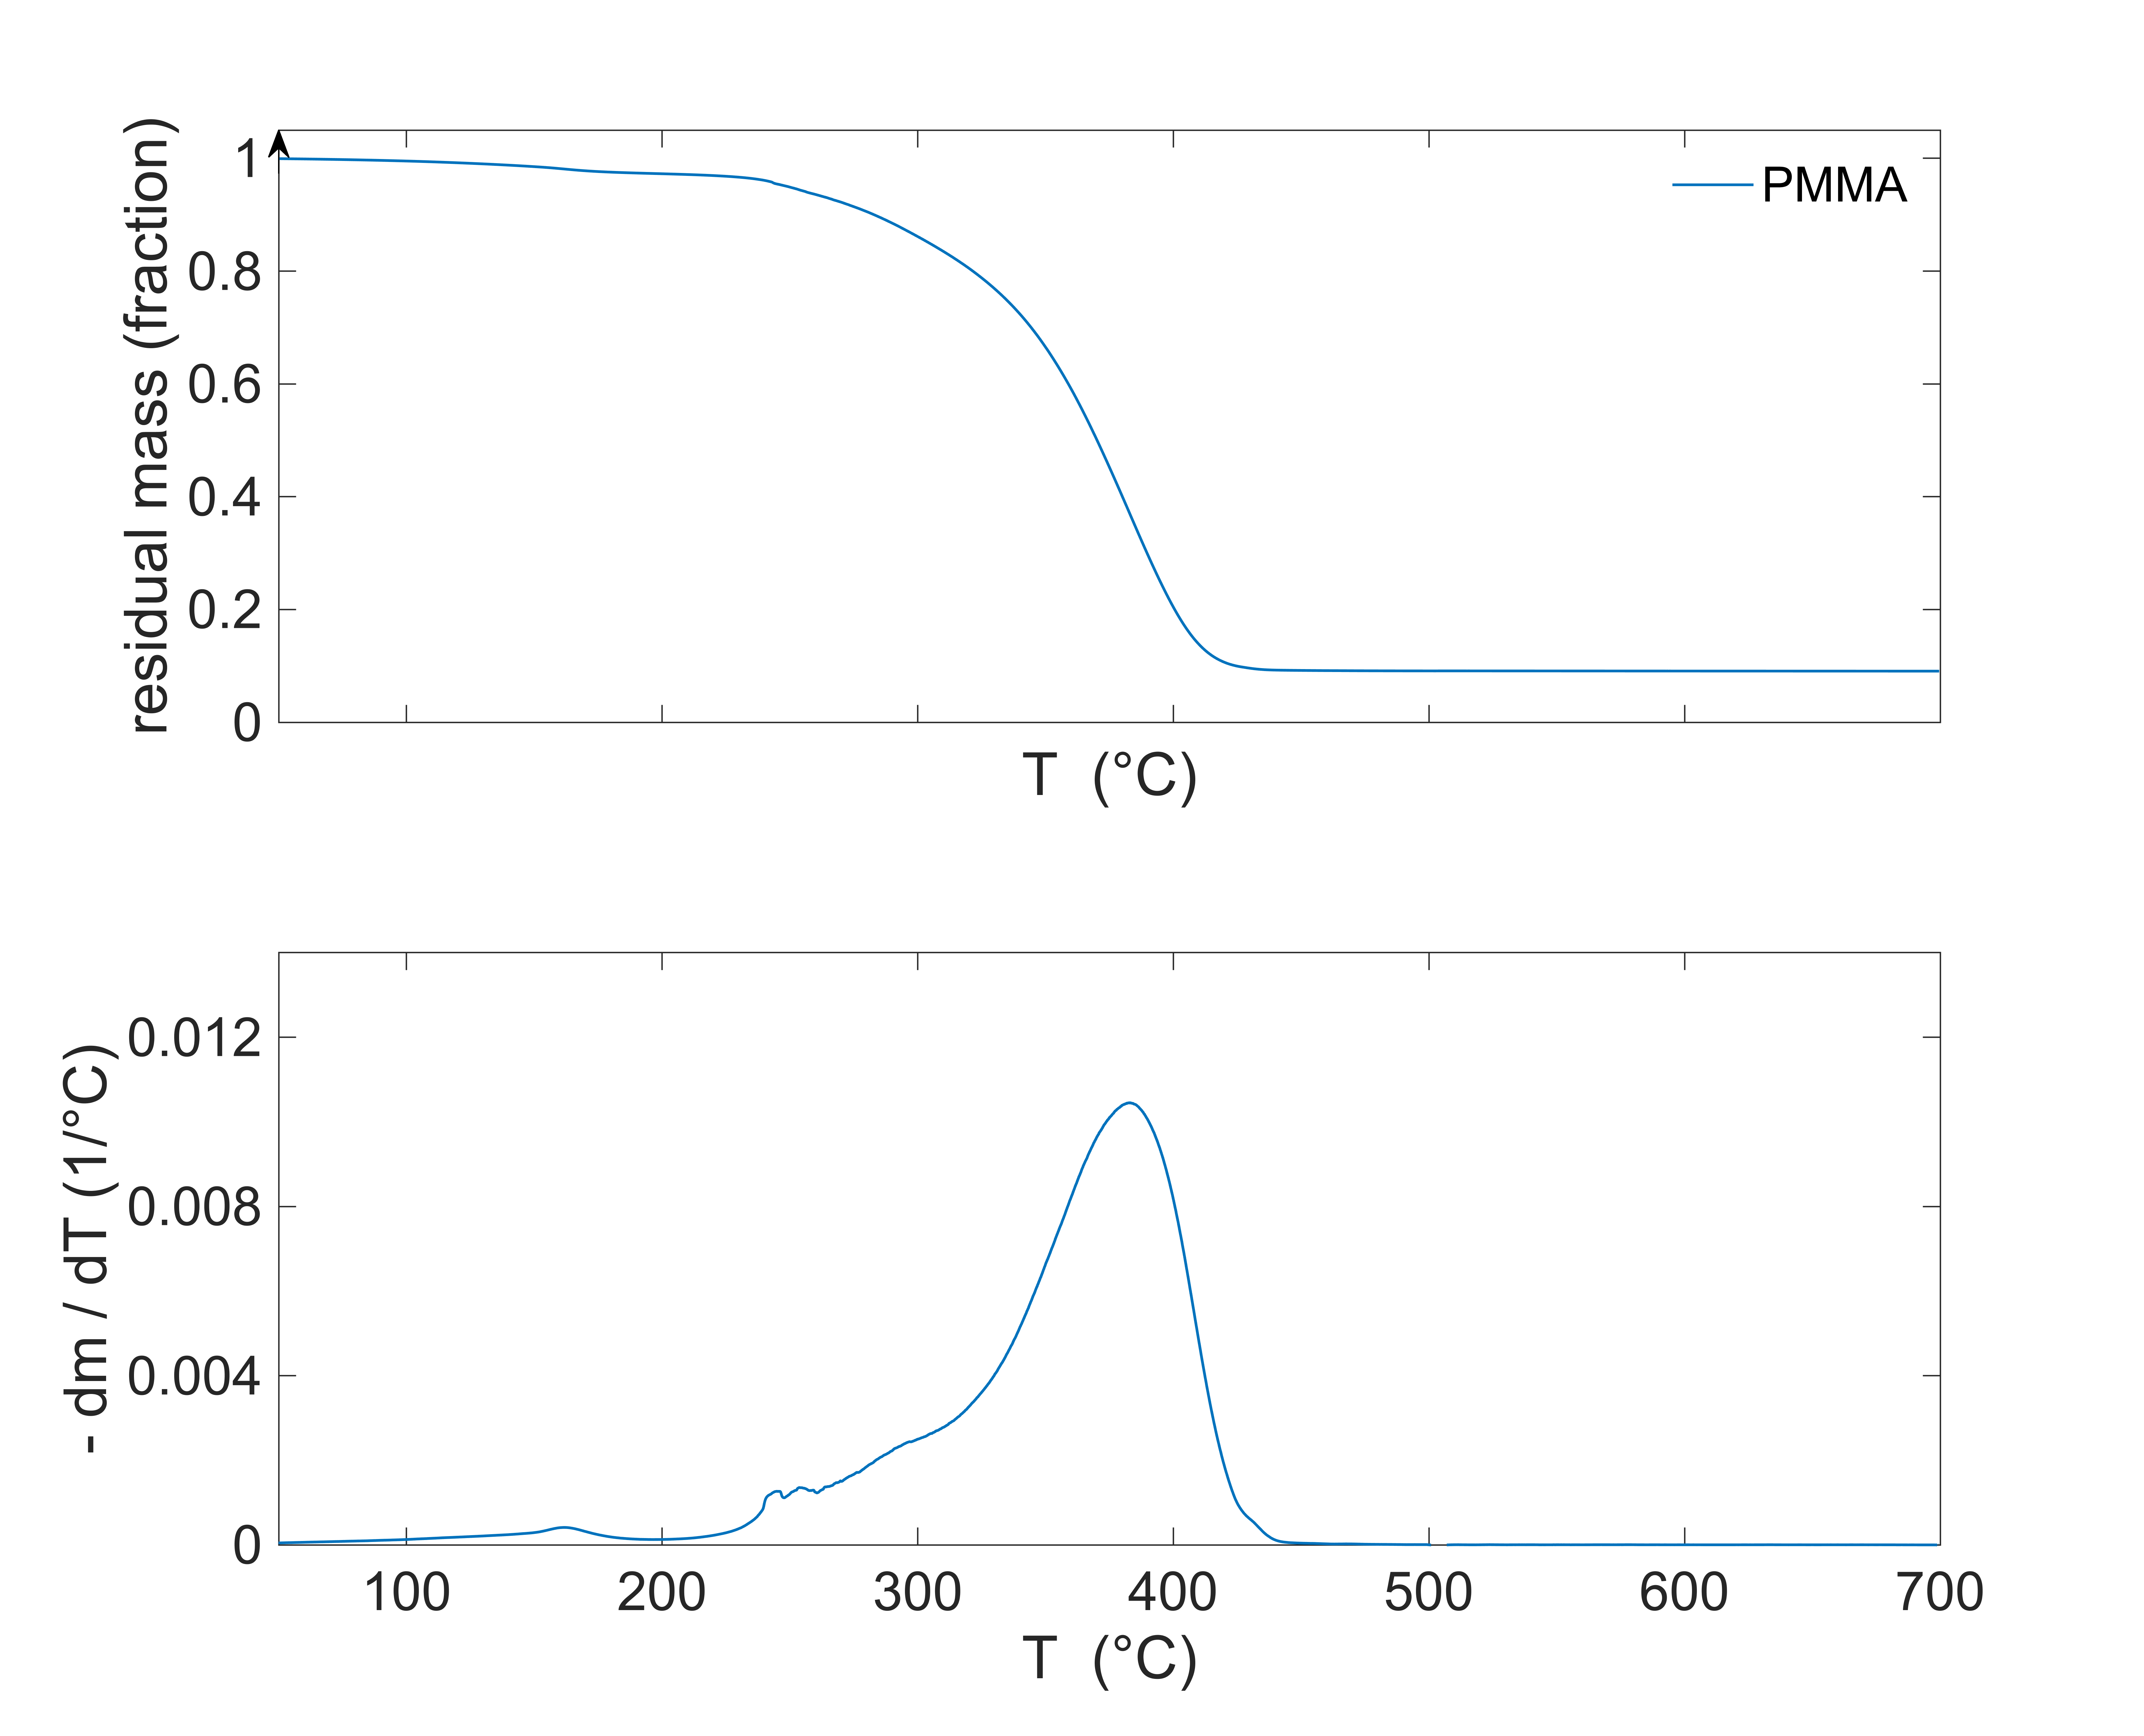
\includegraphics[scale=0.42]{tgaPMMA}} \quad 
\subfloat[][]
{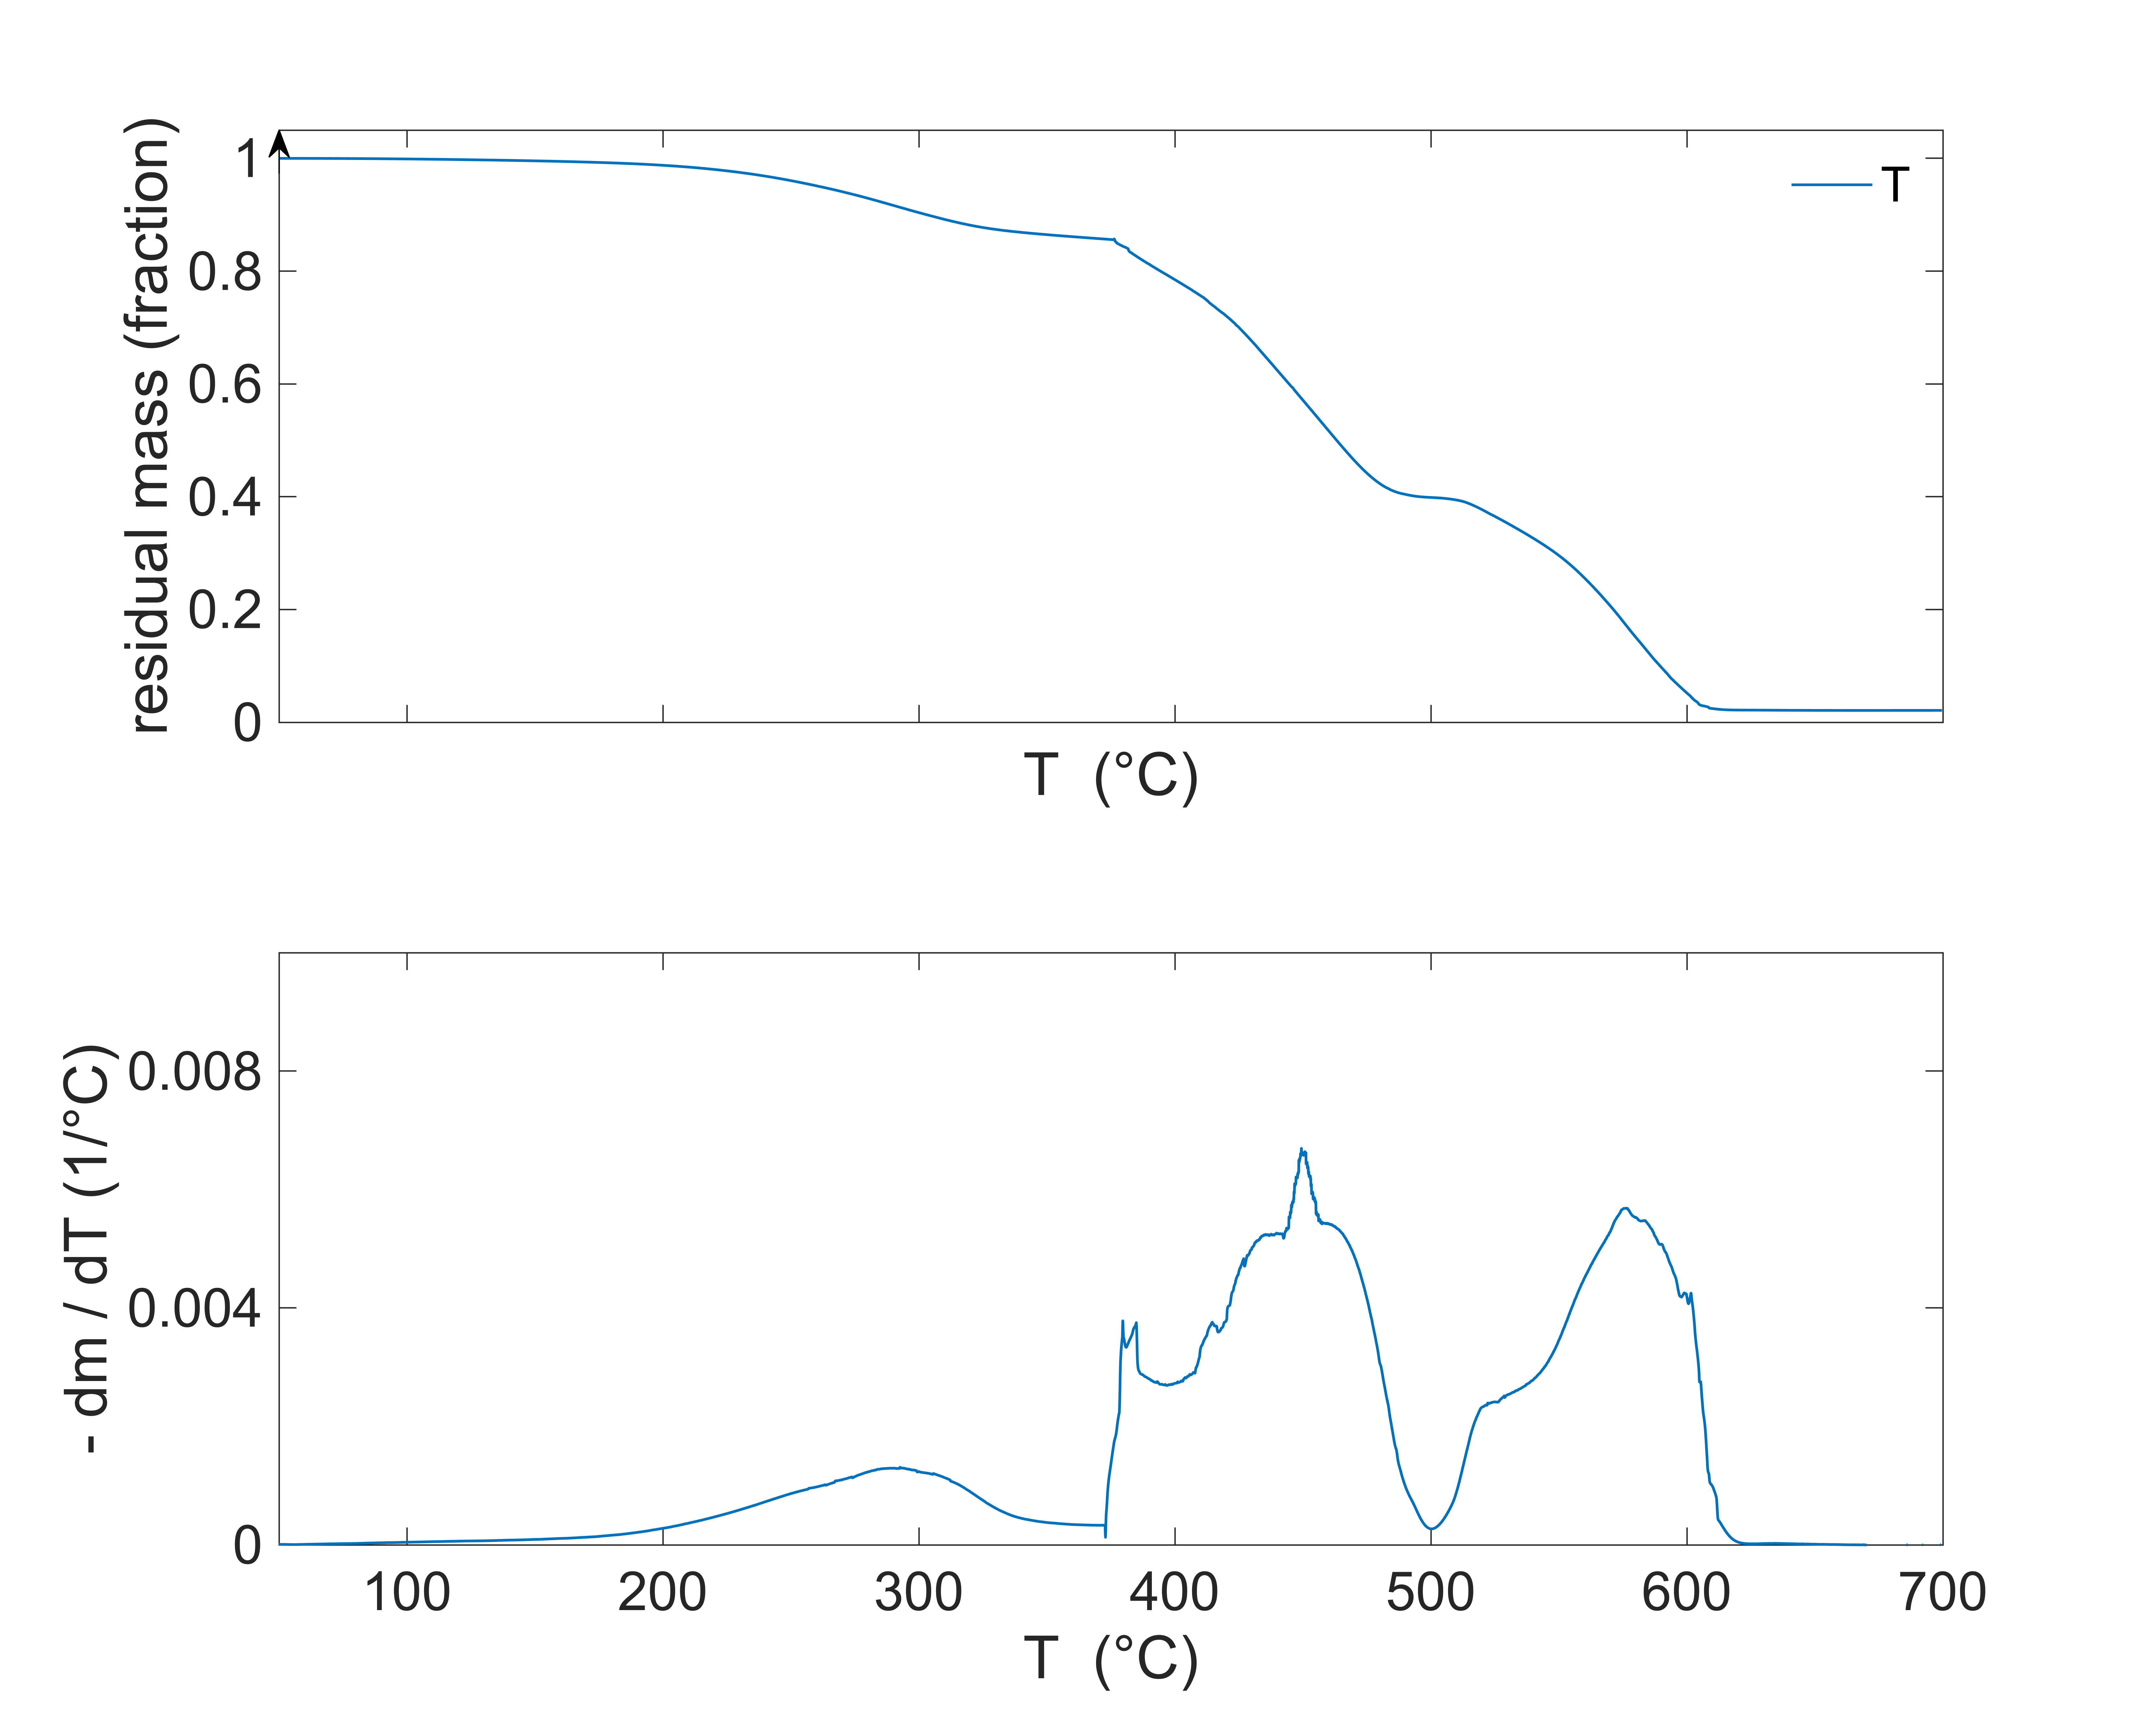
\includegraphics[scale=0.42]{tgaT}} \quad 
\captionsetup{justification=centering}
\caption{TGA thermograms for (a) Bone cement and (b) T samples.}
\label{fig:tga}
\end{figure}\\
From Figure \ref{fig:tga}a it can be noticed that at $161.6^\circ C $ the $2.35 \%$ of the total mass is lost, probably due to presence of water. At $382.9^\circ$C, degradation of the polymer (PMMA) occurs and thus a loss of $87.70\%$ of the initial mass is registered. However a residue of $9.1\%$ is left at the end of the process because the barium sulphate (\chemfig{BaSO_{4}}) is stable as inorganic compound. This percentage of remaining mass is comparable with the value of the amount of sulphate found in the previous laboratory activity that was equal to $9.6\%$ for the first polymerization (P1)~\cite{gruppo1}. 

\newpage

From Figure \ref{fig:tga}b it can be observed that a first loss of mass of about $13.7\%$ is present at $288.8^\circ$C due to volatilization of oils and other chemical products contained in the blend, while in the interval 387.5 – 457.8°C the maximum degradation rate of the rubber is found with a mass loss equal to $45.8\%$. At about $575.9^\circ$C another loss of about $37.5\%$ related to carbon black is seen. In this case a residual mass of $2.1\%$ is left at the end of the analysis. These values of mass losses are comparable with the usual composition of a tire~\cite{gommista}.\\
In Table \ref{tab:tga} results of TGA analysis on all samples are displayed. 
\begin{table}[htp]
\centering
$
\begin{array}{lccccc}
\toprule
\textbf{Sample}  & \bm{T_{d,1}} (\SI{}{\celsius}) & \bm{T_{d,2}} (\SI{}{\celsius}) & \bm{T_{d,3}} (\SI{}{\celsius}) & \bm{T_{d,4}} (\SI{}{\celsius}) & \bm{m_{r}} (\si{\%}) \\
\midrule
\text{PMMA}  & 382.9 & - & - & - & 9.1  \\
\text{T}  & 288.8 & 387.5 & 457.8 & 575.9 & 2.1  \\
\bottomrule
\end{array}
$
\caption{TGA results for all samples. $T_d$ is representative of the maximum rate of mass loss.}
\label{tab:tga}
\end{table}\\
Moreover, it has been evaluated the amount of natural and synthetic rubber present in the sample looking at the thermogram and its derivative: the derivative shows two peaks and the thermogram shows a slight difference in the slope, corresponding to the degradation of the two components. The amount has been extimated as 30\% of natural rubber and 70\% as synthetic rubber. These values of mass losses are comparable with the usal compostion of the tire.

\subsection{Solvent effect}

Polystyrene stick put in ethanol has maintained its features, showing the resistance of polystyrene to this solvent. Sticks put in acetone show different responses depending on the concentration of the solution: in acetone 25\% the specimen is softer but maintains it shape, with a concentration of 50\% the stick is no more intact and the remaining part is spreaded on the sides of the test tubes. Increasing more the concentration (acetone 75\%) the remaining polystyrene stick is less visible until it is completely dissolved by the solvent at the concentration of 100\%. The specimen tested with the mixture of acetone shows an higher resistance to the commercal solvent, due to its lower concentration.
These experimental evidences are in agreement with what expected, acetone can enter in polymer chains and can be absorbed by the stick according to the concentration of the solvent, this is more favorable in the case of polystyrene due to its amorphous structure. The specimen put in the acetone mixture used in cosmetic becomes softer with the possibility to change significantly its shape and once it is deformed, if the solvent is left to evaporate, the specimen maintains the new shape.
Polystyrene shows low resistance also to aromatic diluent that contains toluene, in fact the sticks and the cups filled with this solvent completely dissolved the part in contact. Otherwise the polypropylene cup submitted to the same experiment has maintains its shape and all other features. The polymer shows a higher resistance to this solvent, thanks to its semicrystallinity and therefore its more ordered structure able to reduce the absorption among the polymer chains.

\newpage

\section{Conclusions}

The laboratory session has concerned the evaluation of some characteristic of common polymeric samples, such as cups, coffee sticks or water bottle, in order to compare theoritical values of  differrent polymers with values of industrial products and  to evaluate the composition of this samples.
Through Archimedean test was find out that the density of PET bottle threaded section, crystallized with heat treatment, was lower than the amorphus value of density of PET. This effect of decreasing of density is due to the presence of diethylene glycol in industrial composition, added to reduce cristallizabilty. 
The addition of DEG is also visible in DSC analysis in decreasing of melting point respect to theoritical value of PET. Density values of PET bottle estimated through DSC analysis are a little bit higher than values obtained with Archimedean test since they don't take into account the presence of DEG and are calculated on the basis of pure PET. 
In DSC in PET and PLA heat treated, as expected, the crystallization peak disappears and this is related to the completion of crystallization in heat treatment. 
In heat treatments it has been noticed that samples trying to return back to preform shape in order to reduce stresses introduced in industrial processes. Semicrystalline polymers in which $T_g$ has been overcome in heat treatments has become more opaque due to the increase of cristallinity. 
In TGA anlysis of PMMA at very high temperatures (above  600$^\circ$C) can been noticed the presence of a residual mass due to the addition of barium sulphate in bone cement composition. In TGA thermogram of tire sample has been evalueted the presence
of different products contained in the blend added to the ABS rubber, such as oil and carbon black. Phr of the rubber has been calculated.  

\newpage
\thispagestyle{empty}

\begin{thebibliography}{1}

\bibitem{handbook} Polymer Handbook, J. Brandrup, E.H. Immergut, third edition, Wiley 2003.
\bibitem{gommista} HF. Mark et al. Encyclopedia of Polymer Science and Technology, third edition, Wiley 2014.
\bibitem{densità} ASTM D792 "Standard test methods for density and specific gravity of plastics by displacement".
\bibitem{gruppo1} Radical polymerization and polymer casting for production of bone cement. Water absorption kinetics analysis. Group 1 of PME 2018/19, University of Trento. 

\end{thebibliography}

\newpage

\begin{appendices}

\section{Density measuraments}

\begin{table}[htp]
\centering
$
\begin{array}{lcccc}
\toprule
\textbf{Sample} & \textbf{Specimen} & \textbf{Weight in air}\,(g) & \textbf{Weight in water}\,(g) & \mathbf{\rho}\,(kg/m^{3})\\
\midrule
\text{PET} & \text{a} & 0.7114 & 0.1684 & 1307\\
& \text{b} & 0.8203 & 0.1984 & 1316\\
& \text{c} & 0.8376 & 0.2029 & 1317\\
\midrule
\text{PET–T1} & \text{a} & 0.6929 & 0.1720 &  1327\\
& \text{b} & 0.8050 & 0.2015 & 1331\\
& \text{c} & 0.3537 & 0.0874 & 1325\\
& \text{d} & 0.5248 & 0.1301 & 1326\\
\midrule
\text{PET–T2} & \text{a} & 0.7491 & 0.1888 & 1334\\
& \text{b} & 0.7711 & 0.1959 & 1337\\
& \text{c} & 0.5891 & 0.1499 & 1338\\
\bottomrule
\end{array}
$
\caption{Weight and density measurements of PET bottles with different thermal treatment.}
\label{tab:admt}
\end{table}

\begin{table}[htp]
\centering
$
\begin{array}{lcccc}
\toprule
\textbf{Sample} & \textbf{Specimen} & \textbf{Weight in air}\,(g) & \textbf{Weight in water}\,(g) &  \mathbf{\rho}\,(kg/m^{3})\\
\midrule
\text{pure} & 1 & 1.1579 & 0.1817 & 1183\\
& 2 & 0.8851 & 0.1388 & 1183\\
\midrule
\text{P2} & \text{A} & 3.1649 & 0.6074 & 1235\\
& \text{D} & 4.6149 & 0.9135 & 1244\\
\midrule
\text{P2 after TT} & \text{C} & 2.1841 & 0.4442 & 1252\\
& \text{B} & 2.6498 & 0.5039 & 1232\\
\bottomrule
\end{array}
$
\caption{Weight and density of PMMA samples.}
\label{tab:apmma}
\end{table}

\newpage

\section{DEG effect}

Chart taken from literature~\cite{handbook}.

\begin{figure}[htp]
\centering
{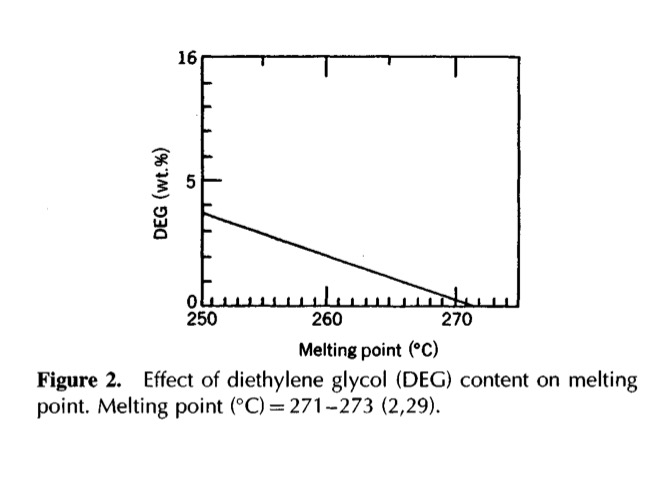
\includegraphics[scale=0.4]{DEG}} \quad 
\captionsetup{justification=centering}
\end{figure}

\end{appendices}

\end{document}